%% LyX 2.4.1 created this file.  For more info, see https://www.lyx.org/.
%% Do not edit unless you really know what you are doing.
\documentclass[journal,article,submit,pdftex,moreauthors]{Definitions/mdpi}
\usepackage[utf8]{inputenc}
\usepackage{float}
\usepackage{url}
\usepackage{graphicx}

\makeatletter

%%%%%%%%%%%%%%%%%%%%%%%%%%%%%% LyX specific LaTeX commands.

\Title{Combining constructed artificial neural networks with parameter constraint
techniques to achieve better generalization properties}

\TitleCitation{Combining constructed artificial neural networks with parameter constraint
techniques to achieve better generalization properties}

\Author{Ioannis G. Tsoulos$^{1,*}$, Vasileios Charilogis$^{2}$, Dimitrios
Tsalikakis$^{3}$}

\AuthorNames{Ioannis G. Tsoulos, Vasileios Charilogis, Dimitrios Tsalikakis}

\AuthorCitation{Tsoulos, I.G.; Charilogis, V.; Tsalikakis D.}


\address{$^{1}$\quad{}Department of Informatics and Telecommunications,
University of Ioannina, Greece;itsoulos@uoi.gr\\
$^{2}$\quad{}Department of Informatics and Telecommunications, University
of Ioannina, Greece; v.charilog@uoi.gr\\
$^{3}\quad$Department of Engineering Informatics and Telecommunications,
University of Western Macedonia, 50100 Kozani, Greece; tsalikakis@gmail.com}


\corres{Correspondence: itsoulos@uoi.gr}


\abstract{This study presents a novel hybrid approach combining grammatical
evolution with constrained genetic algorithms to overcome key limitations
in automated neural network design. The proposed method addresses
two critical challenges: the tendency of grammatical evolution to
converge to suboptimal architectures due to local optima, and the
common overfitting problems in evolved networks. Our solution employs
grammatical evolution for initial architecture generation while implementing
a specialized genetic algorithm that simultaneously optimizes network
parameters within dynamically adjusted bounds. The genetic component
incorporates innovative penalty mechanisms in its fitness function
to control neuron activation patterns and prevent overfitting. Comprehensive
testing across 53 diverse datasets shows our method achieves superior
performance compared to traditional optimization techniques, with
an average classification error of 21.18\% versus 36.45\% for ADAM,
while maintaining better generalization capabilities. The constrained
optimization approach proves particularly effective in preventing
premature convergence, and the penalty system successfully mitigates
overfitting even in complex, high-dimensional problems. Statistical
validation confirms these improvements are significant (p \textless{}
1.1e-08) and consistent across multiple domains including medical
diagnosis, financial prediction, and physical system modeling. This
work provides a robust framework for automated neural network construction
that balances architectural innovation with parameter optimization
while addressing fundamental challenges in evolutionary machine learning.}


\keyword{Grammatical Evolution; Genetic Programming; Neural networks; Local
Optimization}

\newcommand*\LyXZeroWidthSpace{\hspace{0pt}}
\DeclareTextSymbolDefault{\textquotedbl}{T1}
%% Because html converters don't know tabularnewline
\providecommand{\tabularnewline}{\\}
\floatstyle{ruled}
\newfloat{algorithm}{tbp}{loa}
\providecommand{\algorithmname}{Algorithm}
\floatname{algorithm}{\protect\algorithmname}

%%%%%%%%%%%%%%%%%%%%%%%%%%%%%% Textclass specific LaTeX commands.
\newenvironment{lyxcode}
	{\par\begin{list}{}{
		\setlength{\rightmargin}{\leftmargin}
		\setlength{\listparindent}{0pt}% needed for AMS classes
		\raggedright
		\setlength{\itemsep}{0pt}
		\setlength{\parsep}{0pt}
		\normalfont\ttfamily}%
	 \item[]}
	{\end{list}}

%%%%%%%%%%%%%%%%%%%%%%%%%%%%%% User specified LaTeX commands.
%  LaTeX support: latex@mdpi.com 
%  For support, please attach all files needed for compiling as well as the log file, and specify your operating system, LaTeX version, and LaTeX editor.

%=================================================================


% For posting an early version of this manuscript as a preprint, you may use "preprints" as the journal and change "submit" to "accept". The document class line would be, e.g., \documentclass[preprints,article,accept,moreauthors,pdftex]{mdpi}. This is especially recommended for submission to arXiv, where line numbers should be removed before posting. For preprints.org, the editorial staff will make this change immediately prior to posting.

%--------------------
% Class Options:
%--------------------
%----------
% journal
%----------
% Choose between the following MDPI journals:
% acoustics, actuators, addictions, admsci, adolescents, aerospace, agriculture, agriengineering, agronomy, ai, algorithms, allergies, alloys, analytica, animals, antibiotics, antibodies, antioxidants, applbiosci, appliedchem, appliedmath, applmech, applmicrobiol, applnano, applsci, aquacj, architecture, arts, asc, asi, astronomy, atmosphere, atoms, audiolres, automation, axioms, bacteria, batteries, bdcc, behavsci, beverages, biochem, bioengineering, biologics, biology, biomass, biomechanics, biomed, biomedicines, biomedinformatics, biomimetics, biomolecules, biophysica, biosensors, biotech, birds, bloods, blsf, brainsci, breath, buildings, businesses, cancers, carbon, cardiogenetics, catalysts, cells, ceramics, challenges, chemengineering, chemistry, chemosensors, chemproc, children, chips, cimb, civileng, cleantechnol, climate, clinpract, clockssleep, cmd, coasts, coatings, colloids, colorants, commodities, compounds, computation, computers, condensedmatter, conservation, constrmater, cosmetics, covid, crops, cryptography, crystals, csmf, ctn, curroncol, currophthalmol, cyber, dairy, data, dentistry, dermato, dermatopathology, designs, diabetology, diagnostics, dietetics, digital, disabilities, diseases, diversity, dna, drones, dynamics, earth, ebj, ecologies, econometrics, economies, education, ejihpe, electricity, electrochem, electronicmat, electronics, encyclopedia, endocrines, energies, eng, engproc, ent, entomology, entropy, environments, environsciproc, epidemiologia, epigenomes, est, fermentation, fibers, fintech, fire, fishes, fluids, foods, forecasting, forensicsci, forests, foundations, fractalfract, fuels, futureinternet, futureparasites, futurepharmacol, futurephys, futuretransp, galaxies, games, gases, gastroent, gastrointestdisord, gels, genealogy, genes, geographies, geohazards, geomatics, geosciences, geotechnics, geriatrics, hazardousmatters, healthcare, hearts, hemato, heritage, highthroughput, histories, horticulturae, humanities, humans, hydrobiology, hydrogen, hydrology, hygiene, idr, ijerph, ijfs, ijgi, ijms, ijns, ijtm, ijtpp, immuno, informatics, information, infrastructures, inorganics, insects, instruments, inventions, iot, j, jal, jcdd, jcm, jcp, jcs, jdb, jeta, jfb, jfmk, jimaging, jintelligence, jlpea, jmmp, jmp, jmse, jne, jnt, jof, joitmc, jor, journalmedia, jox, jpm, jrfm, jsan, jtaer, jzbg, kidney, kidneydial, knowledge, land, languages, laws, life, liquids, literature, livers, logics, logistics, lubricants, lymphatics, machines, macromol, magnetism, magnetochemistry, make, marinedrugs, materials, materproc, mathematics, mca, measurements, medicina, medicines, medsci, membranes, merits, metabolites, metals, meteorology, methane, metrology, micro, microarrays, microbiolres, micromachines, microorganisms, microplastics, minerals, mining, modelling, molbank, molecules, mps, msf, mti, muscles, nanoenergyadv, nanomanufacturing, nanomaterials, ncrna, network, neuroglia, neurolint, neurosci, nitrogen, notspecified, nri, nursrep, nutraceuticals, nutrients, obesities, oceans, ohbm, onco, oncopathology, optics, oral, organics, organoids, osteology, oxygen, parasites, parasitologia, particles, pathogens, pathophysiology, pediatrrep, pharmaceuticals, pharmaceutics, pharmacoepidemiology, pharmacy, philosophies, photochem, photonics, phycology, physchem, physics, physiologia, plants, plasma, pollutants, polymers, polysaccharides, poultry, powders, preprints, proceedings, processes, prosthesis, proteomes, psf, psych, psychiatryint, psychoactives, publications, quantumrep, quaternary, qubs, radiation, reactions, recycling, regeneration, religions, remotesensing, reports, reprodmed, resources, rheumato, risks, robotics, ruminants, safety, sci, scipharm, seeds, sensors, separations, sexes, signals, sinusitis, skins, smartcities, sna, societies, socsci, software, soilsystems, solar, solids, sports, standards, stats, stresses, surfaces, surgeries, suschem, sustainability, symmetry, synbio, systems, taxonomy, technologies, telecom, test, textiles, thalassrep, thermo, tomography, tourismhosp, toxics, toxins, transplantology, transportation, traumacare, traumas, tropicalmed, universe, urbansci, uro, vaccines, vehicles, venereology, vetsci, vibration, viruses, vision, waste, water, wem, wevj, wind, women, world, youth, zoonoticdis 

%---------
% article
%---------
% The default type of manuscript is "article", but can be replaced by: 
% abstract, addendum, article, book, bookreview, briefreport, casereport, comment, commentary, communication, conferenceproceedings, correction, conferencereport, entry, expressionofconcern, extendedabstract, datadescriptor, editorial, essay, erratum, hypothesis, interestingimage, obituary, opinion, projectreport, reply, retraction, review, perspective, protocol, shortnote, studyprotocol, systematicreview, supfile, technicalnote, viewpoint, guidelines, registeredreport, tutorial
% supfile = supplementary materials

%----------
% submit
%----------
% The class option "submit" will be changed to "accept" by the Editorial Office when the paper is accepted. This will only make changes to the frontpage (e.g., the logo of the journal will get visible), the headings, and the copyright information. Also, line numbering will be removed. Journal info and pagination for accepted papers will also be assigned by the Editorial Office.

%------------------
% moreauthors
%------------------
% If there is only one author the class option oneauthor should be used. Otherwise use the class option moreauthors.

%---------
% pdftex
%---------
% The option pdftex is for use with pdfLaTeX. If eps figures are used, remove the option pdftex and use LaTeX and dvi2pdf.

%=================================================================
% MDPI internal commands - do not modify
\firstpage{1} 
 
\setcounter{page}{\@firstpage} 

\pubvolume{1}
\issuenum{1}
\articlenumber{0}
\pubyear{2024}
\copyrightyear{2024}
%\externaleditor{Academic Editor: Firstname Lastname} % For journal Automation, please change Academic Editor to "Communicated by"
\datereceived{}
\daterevised{ } % Comment out if no revised date
\dateaccepted{}
\datepublished{}
%\datecorrected{} % Corrected papers include a "Corrected: XXX" date in the original paper.
%\dateretracted{} % Corrected papers include a "Retracted: XXX" date in the original paper.
\hreflink{https://doi.org/} % If needed use \linebreak
%\doinum{}
%------------------------------------------------------------------
% The following line should be uncommented if the LaTeX file is uploaded to arXiv.org
%\pdfoutput=1

%=================================================================
% Add packages and commands here. The following packages are loaded in our class file: fontenc, inputenc, calc, indentfirst, fancyhdr, graphicx, epstopdf, lastpage, ifthen, lineno, float, amsmath, setspace, enumitem, mathpazo, booktabs, titlesec, etoolbox, tabto, xcolor, soul, multirow, microtype, tikz, totcount, changepage, attrib, upgreek, cleveref, amsthm, hyphenat, natbib, hyperref, footmisc, url, geometry, newfloat, caption

%=================================================================
%% Please use the following mathematics environments: Theorem, Lemma, Corollary, Proposition, Characterization, Property, Problem, Example, ExamplesandDefinitions, Hypothesis, Remark, Definition, Notation, Assumption
%% For proofs, please use the proof environment (the amsthm package is loaded by the MDPI class).

%=================================================================
% The fields PACS, MSC, and JEL may be left empty or commented out if not applicable
%\PACS{J0101}
%\MSC{}
%\JEL{}

%%%%%%%%%%%%%%%%%%%%%%%%%%%%%%%%%%%%%%%%%%
% Only for the journal Diversity
%\LSID{\url{http://}}

%%%%%%%%%%%%%%%%%%%%%%%%%%%%%%%%%%%%%%%%%%
% Only for the journal Applied Sciences:
%\featuredapplication{Authors are encouraged to provide a concise description of the specific application or a potential application of the work. This section is not mandatory.}
%%%%%%%%%%%%%%%%%%%%%%%%%%%%%%%%%%%%%%%%%%

%%%%%%%%%%%%%%%%%%%%%%%%%%%%%%%%%%%%%%%%%%
% Only for the journal Data:
%\dataset{DOI number or link to the deposited data set in cases where the data set is published or set to be published separately. If the data set is submitted and will be published as a supplement to this paper in the journal Data, this field will be filled by the editors of the journal. In this case, please make sure to submit the data set as a supplement when entering your manuscript into our manuscript editorial system.}

%\datasetlicense{license under which the data set is made available (CC0, CC-BY, CC-BY-SA, CC-BY-NC, etc.)}

%%%%%%%%%%%%%%%%%%%%%%%%%%%%%%%%%%%%%%%%%%
% Only for the journal Toxins
%\keycontribution{The breakthroughs or highlights of the manuscript. Authors can write one or two sentences to describe the most important part of the paper.}

%%%%%%%%%%%%%%%%%%%%%%%%%%%%%%%%%%%%%%%%%%
% Only for the journal Encyclopedia
%\encyclopediadef{Instead of the abstract}
%\entrylink{The Link to this entry published on the encyclopedia platform.}
%%%%%%%%%%%%%%%%%%%%%%%%%%%%%%%%%%%%%%%%%%

%%%%%%%%%%%%%%%%%%%%%%%%%%%%%%%%%%%%%%%%%%
% Only for the journal Advances in Respiratory Medicine
%\addhighlights{yes}
%\renewcommand{\addhighlights}{%

%\noindent This is an obligatory section in “Advances in Respiratory Medicine”, whose goal is to increase the discoverability and readability of the article via search engines and other scholars. Highlights should not be a copy of the abstract, but a simple text allowing the reader to quickly and simplified find out what the article is about and what can be cited from it. Each of these parts should be devoted up to 2~bullet points.\vspace{3pt}\\
%\textbf{What are the main findings?}
% \begin{itemize}[labelsep=2.5mm,topsep=-3pt]
% \item First bullet.
% \item Second bullet.
% \end{itemize}\vspace{3pt}
%\textbf{What is the implication of the main finding?}
% \begin{itemize}[labelsep=2.5mm,topsep=-3pt]
% \item First bullet.
% \item Second bullet.
% \end{itemize}
%}
%%%%%%%%%%%%%%%%%%%%%%%%%%%%%%%%%%%%%%%%%%

\makeatother

\begin{document}
\maketitle

\section{Introduction}

A basic machine learning technique with a wide range of applications
in data classification and regression problems is artificial neural
networks \citep{nn1,nn2}. Artificial neural networks are parametric
machine learning model, in which learning is achieved by effectively
adjusting their parameters through any optimization technique. The
optimization procedure minimizes the so - called training error of
an artificial neural network and it is defined as: 
\begin{equation}
E\left(N\left(\overrightarrow{x},\overrightarrow{w}\right)\right)=\sum_{i=1}^{M}\left(N\left(\overrightarrow{x}_{i},\overrightarrow{w}\right)-y_{i}\right)^{2}\label{eq:eq1}
\end{equation}
In this equation the function $N\left(\overrightarrow{x},\overrightarrow{w}\right)$
represents the artificial neural network which is applied on a vector
$\overrightarrow{x}$ and the vector $\overrightarrow{w}$ denotes
the parameter vector of the neural network. The set $\left(\overrightarrow{x_{i}},y_{i}\right),\ i=1,...,M$
represents the training set of the objective problem and the values
$y_{i}$ are the expected outputs for each pattern $\overrightarrow{x_{i}}$. 

Artificial neural networks have been applied in a wide series of problems
appeared in real - world problems, such as image processing \citep{nn_image},
time series forecasting \citep{nn_timeseries}, credit card analysis
\citep{nn_credit}, problems derived from physics \citep{nnphysics1,nnphysics2}
etc. Due to the widespread use of these machine learning models, a
number of techniques have been proposed to minimize the equation \ref{eq:eq1},
such as the Back Propagation algorithm \citep{bpnn1,bpnn2}, the RPROP
algorithm \citep{rpropnn-1,rpropnn-2}, the ADAM optimization method
\citep{nn_adam} etc. Also, recently a series of more advanced global
optimization methods have been proposed to tackle the training of
neural networks. Among them one can locate the incorporation of Genetic
Algorithms \citep{geneticnn1}, the usage of the Particle Swarm Optimization
(PSO) method \citep{psonn}, the Simulated Annealing method \citep{nn_siman},
the Differential Evolution technique \citep{weight_de1}, the Artificial
Bee Colony (ABC) method \citep{nn_abc} etc. Furthermore, Sexton et
al suggested the usage of the tabu search algorithm for optimal neural
network training \citep{tabunn}, Zhang et al proposed a hybrid algorithm
that incorporated the PSO method and the Back Propagation algorithm
to efficient train artificial neural networks \citep{nn_hybrid}.
Also, recently Zhao et al introduced a new Cascaded Forward Algorithm
to train artificial neural networks \citep{nn_cascade}. Furthermore,
due to the rapid spread of the use of parallel computing techniques,
a series of computational techniques have emerged that exploit parallel
computing structures for faster training of artificial neural networks
\citep{nn_gpu1,nn_gpu2}.

However, the above techniques, although extremely effective, nevertheless
have a number of problems such as, for example, trapping in local
minima of the error function or the phenomenon of overifitting, where
the artificial neural network exhibits reduced performance when applied
to data that was not present during the training process. The overfitting
problem has been studied by many researchers that have proposed a
series of methods to handle this problem, such as weight sharing \citep{nnsharing1,nnsharing2},
pruning \citep{nnprunning1,nnprunning2}, early stopping \citep{nnearly1,nnearly2},
weight decaying \citep{nndecay1,nndecay2} etc. Also, many researchers
propose as a solution to the above problem the dynamic creation of
the architecture of artificial neural networks using programming techniques.
For example the Genetic Algorithms were proposed to create dynamically
the optimal architecture of neural networks \citep{nn_arch1,nn_arch2}
or the PSO method \citep{nn_arch3}.\textbf{ }Siebel et al, suggested
the usage of evolutionary reinforcement learning for the optimal design
of artificial neural networks \citep{nn_ereinf}. Also, Jaafra et
al provided a review on the usage of Reinforcement learning for neural
architecture search \citep{nn_reinf}. In the same direction of research,
Pham et al proposed a method for efficient identification of the architecture
of neural networks through parameters sharing \citep{nn_param_sharing}.
Also, the method of Stochastic Neural Architecture search was suggested
by Xie et al in a recent publication \citep{nn_snas}. Moreover, Zhou
et al introduced a Bayesian approach for neural architecture search
\citep{nn_bayes}.

Recently, genetic algorithms have been incorporated to identify the
optimal set of parameters of neural networks for drug discovery \citep{nn_drug}.
Kim et al proposed \citep{nn_estimates} genetic algorithms to train
neural networks for predicting preliminary cost estimates. Moreover,
Kalogirou proposed the usage of genetic algorithms for effective training
of neural networks for the optimization of solar systems \citep{nn_solar}.
The ability of neural networks to perform feature selection with the
assistance of genetic algorithms was also studied in the work of Tong
et al \citep{nn_feature}. Recently, Ruehle provided a study of the
string landscape using genetic algorithms to train artificial neural
networks \citep{nn_string}.

A method that was proposed relatively recently and it is based on
Grammatical Evolution \citep{ge1}, dynamically identifies both the
optimal architecture of artificial neural networks and the optimal
values of its parameters \citep{nnc}. This method has been applied
in a series of problems in the recent literature, such as problems
presented in chemistry \citep{nnc_amide1}, identification of the
solution of differential equations \citep{nnc_de}, medical problems
\citep{nnc_feas}, problems related to education \citep{nnc_student},
autism screening \citep{nnc_autism} etc. A key advantage of this
technique is that it can isolate from the initial features of the
problem those that are most important in training the model, thus
significantly reducing the required number of parameters that need
to be identified.

However, the method of constructing artificial neural networks can
easily get trapped in local minima of the training error since it
does not have any technique to avoid them. Furthermore, although the
method can get quite close to a minimum of the training error, it
often does not reach it since there is no technique in the method
to train the generated parameters. In this technique, it is proposed
to enhance the original method of constructing artificial neural networks
by periodically applying a modified genetic algorithm to randomly
selected chromosomes of Grammatical Evolution. This modified genetic
algorithm preserves the architecture created by the Grammatical Evolution
method and effectively locates the parameters of the artificial neural
network by reducing the training error. In addition, the proposed
genetic algorithm through appropriate penalty factors imposed on the
fitness function prevents the artificial neural network from overfitting.

The motivation of the proposed method is the need to address two main
challenges in training artificial neural networks: getting trapped
in local minima and the phenomenon of overfitting. Getting trapped
in local minima limits the model's ability to minimize training error,
leading to poor performance on test data. Overfitting similarly reduces
generalization, as the model adapts excessively to the training data.
The proposed method combines Grammatical Evolution with a modified
genetic algorithm to address these problems. Grammatical Evolution
is used for the dynamic construction of the neural network's architecture,
while the genetic algorithm optimizes the network's parameters while
preserving its structure. Additionally, penalty factors are introduced
in the cost function to prevent overfitting. A key innovation is the
use of an algorithm that measures the network's tendency to lose generalization
capability when neuron activations become saturated. This is achieved
by monitoring the input values of the sigmoid function and imposing
penalties when they exceed a specified range. Experimental tests showed
that the method outperforms other techniques such as ADAM, BFGS, and
RBF networks, in both classification and regression problems. Statistical
analysis confirmed the significant improvement in performance, with
very low p-values in the comparisons.

For the suggested work, the main contributions are as follows:
\begin{enumerate}
\item A novel hybrid framework that effectively combines grammatical evolution
for neural architecture search with constrained genetic algorithms
for parameter optimization, addressing both structural design and
weight training simultaneously.
\item An innovative penalty mechanism within the genetic algorithm's fitness
function that dynamically monitors and controls neuron activation
patterns to prevent overfitting, demonstrated to reduce test error
by an average of 15.27\% compared to standard approaches.
\item Comprehensive experimental validation across 53 diverse datasets showing
statistically significant improvements ($p<1.1\times10^{-8}$) over
traditional optimization methods, with particular effectiveness in
medical and financial domains where overfitting risks are critical.
\item Detailed analysis of the method's computational characteristics and
scalability, providing practical guidelines for implementation in
real-world scenarios with resource constraints.
\end{enumerate}
Although the method can construct the correct network structure, its
parameters often remain suboptimal. This means the network fails to
fully exploit its architecture's potential, resulting in lower performance
compared to other approaches. Furthermore, the absence of efficient
training mechanisms leads to increased training times, making the
method less practical for applications requiring quick results. In
specific application scenarios, these limitations become even more
apparent. For instance, with high-dimensional data, the method struggles
to identify relationships between features while computational times
become prohibitive. With limited training data, the constructed networks
tend to overfit, resulting in poor generalization to new data. For
real-time applications, the high computational complexity makes the
method impractical. Compared to other approaches like traditional
neural networks with backpropagation, modern deep learning architectures,
or meta-learning methods, grammatical evolution appears inferior in
several aspects. It requires significantly more computational resources,
consistently achieves lower performance, and presents scalability
limitations. These factors restrict the method's application in production
systems where stability and result predictability are crucial. The
practical implications of these limitations are substantial. The method
requires extensive hyperparameter tuning to produce acceptable results,
while its performance can be unpredictable and vary significantly
between different runs. For successful application to real-world problems,
additional processing and result validation are often necessary. Despite
its limitations, the method offers interesting capabilities for the
automatic construction of neural network architectures. However, to
become truly competitive against existing approaches, it requires
the development of more sophisticated optimization algorithms to reduce
local minima trapping, the integration of efficient parameter training
mechanisms, and improvements in method scalability. Only by addressing
these issues can grammatical evolution emerge as an attractive alternative
in the field of automated neural network design.

The remaining of this article is organized as follows: in section
\ref{sec:Method-description} the proposed method and the accompanied
genetic algorithm are introduced, in section \ref{sec:Results} the
experimental datasets and the series of experiments conducted are
listed and discussed thoroughly followed by the section \ref{sec:Discussion},
where a discussion on the experimental results is provided and final
in section \ref{sec:Conclusions} some conclusions are discussed.

\section{Method description\protect\label{sec:Method-description}}

This section provides a details description of the original neural
network construction method and continuous with the proposed genetic
algorithm and concludes with the overall algorithm.

\subsection{The neural construction method \protect\label{subsec:The-neural-construction}}

The neural construction method utilizes the technique of Grammatical
Evolution to produce artificial neural networks. Grammatical Evolution
is an evolutionary process where the chromosomes are vectors of positive
integers. These integers represent rules from a Backs - Naur form
(BNF) grammar \citep{bnf1} of the target language.\textbf{ }The method
was incorporated in various cases, such as data fitting\textbf{ }\citep{ge_program1,ge_program2},
composition of music \citep{ge_music}, video games \citep{ge_pacman,ge_supermario},
energy problems \citep{ge_energy}, cryptography \citep{ge_crypt},
economics \citep{ge_trading} etc. Any BNF grammar is defined as a
set\textbf{ $G=\left(N,T,S,P\right)$ }where the letters have the
following definitions:
\begin{itemize}
\item The set $N$ represents the non - terminal symbols of the grammar.
\item The set $T$ contains the terminal symbols of the grammar. 
\item The start symbol of the grammar is denoted as $S$.
\item The production rules of the grammar are enclosed in the set $P$
\end{itemize}
The Grammatical Evolution production procedure initiates from the
starting symbol $S$ and following a series of steps, the method creates
valid programs by replacing non-terminal symbols with the right hand
of the selected production rule. The selection scheme has as:
\begin{itemize}
\item \textbf{Read} the next element V from the chromosome that is being
processed.
\item \textbf{Select} the next production rule following the equation:Rule
= V mod $N_{R}$. The symbol $N_{R}$ represents the total number
of production rules for the under processing non -- terminal symbol. 
\end{itemize}
The process of producing valid programs through the Grammatical Evolution
method is depicted graphically in Figure \ref{fig:geProcess}.

\begin{figure}[H]
\begin{centering}

\includegraphics[scale=0.5]{GEFC}
\par\end{centering}
\caption{The Grammatical Evolution process used to produce valid programs.\protect\label{fig:geProcess}}

\end{figure}
The grammar used for the neural construction procedure is shown in
Figure \ref{fig:nncGrammar}. The numbers shown in parentheses are
the increasing numbers of the production rules for each non - terminal
symbol. The constant $d$ denotes the number of features in every
pattern of the input dataset.

\begin{figure}[H]
\begin{lyxcode}
S:=\textless Sigval\textgreater ~~~~~~~~~~~~~~~~~~~~~~~~~~(0)

\textless Sigval\textgreater ::=\textless Node\textgreater ~~~~~~~~~~~~~~~~~~~~(0)

~~~~~~~~~~~\textbar ~\textless Node\textgreater ~+~\textless Sigval\textgreater ~~~~~~~(1)

\textless Node\textgreater ::=\textless Number\textgreater{*}sig(\textless Sum\textgreater +\textless Number\textgreater )~(0)

\textless Sum\textgreater ::=~\textless Number\textgreater{*}\textless Xlist\textgreater ~~~~~~~~~~~~(0)

~~~~~~~~~~~\textbar ~~~~\textless Sum\textgreater +\textless Sum\textgreater ~~~~~~~~~~~(1)

\textless Xlist\textgreater ::=~x1~~~~~~~~(0)

~~~~~~~~~~~~~\textbar ~~~~x2~~(1)

~~~~~~~~~~~~~..............

~~~~~~~~~~~~~\textbar ~~~~xd~~(d-1)

\textless Number\textgreater ::=~(\textless Dlist\textgreater .\textless Dlist\textgreater )~~~~~~~~(0)

~~~~~~~~~~~~~\textbar ~~~~(-\textless Dlist\textgreater .\textless Dlist\textgreater )~(1)

\textless Dlist\textgreater ::=~\textless Digit\textgreater ~~~~~~~~~~~~(0)

~~~~~~~~~~~~~\textbar ~\textless Digit\textgreater\textless Dlist\textgreater ~(1)

\textless Digit\textgreater ::=~0~~~~~~(0)

~~~~~~~~~~~~~\textbar ~~1~(1)

~~~~~~~~~~~~~...........

~~~~~~~~~~~~~\textbar ~~9~(9)
\end{lyxcode}
\caption{The proposed grammar for the construction of artificial neural networks
through Grammatical Evolution.\protect\label{fig:nncGrammar}}
\end{figure}
The used grammar produces artificial neural networks with the following
form:

\begin{equation}
N\left(\overrightarrow{x},\overrightarrow{w}\right)=\sum_{i=1}^{H}w_{(d+2)i-(d+1)}\sigma\left(\sum_{j=1}^{d}x_{j}w_{(d+2)i-(d+1)+j}+w_{(d+2)i}\right)\label{eq:nn}
\end{equation}
The term $H$ stands for the number of processing units (weights)
of the neural network. The function $\sigma(x)$ represents the sigmoid
function.\textbf{ }The total number of parameters for this network
are computed through the following equation:
\begin{equation}
n=\left(d+2\right)H
\end{equation}
For example the following form:
\begin{equation}
N(x)=1.9\mbox{sig}\left(10.5x_{1}+3.2x_{3}+1.4\right)+2.1\mbox{sig}\left(2.2x_{2}-3.3x_{3}+3.2\right)
\end{equation}
denotes a produced neural network for a problem with 3 inputs $\left(x_{1},x_{2},x_{3}\right)$
and the number of processing nodes is $H=2$. The neural network produced
can be shown graphically in Figure \ref{fig:nnExample}.

\begin{figure}[H]
\begin{centering}
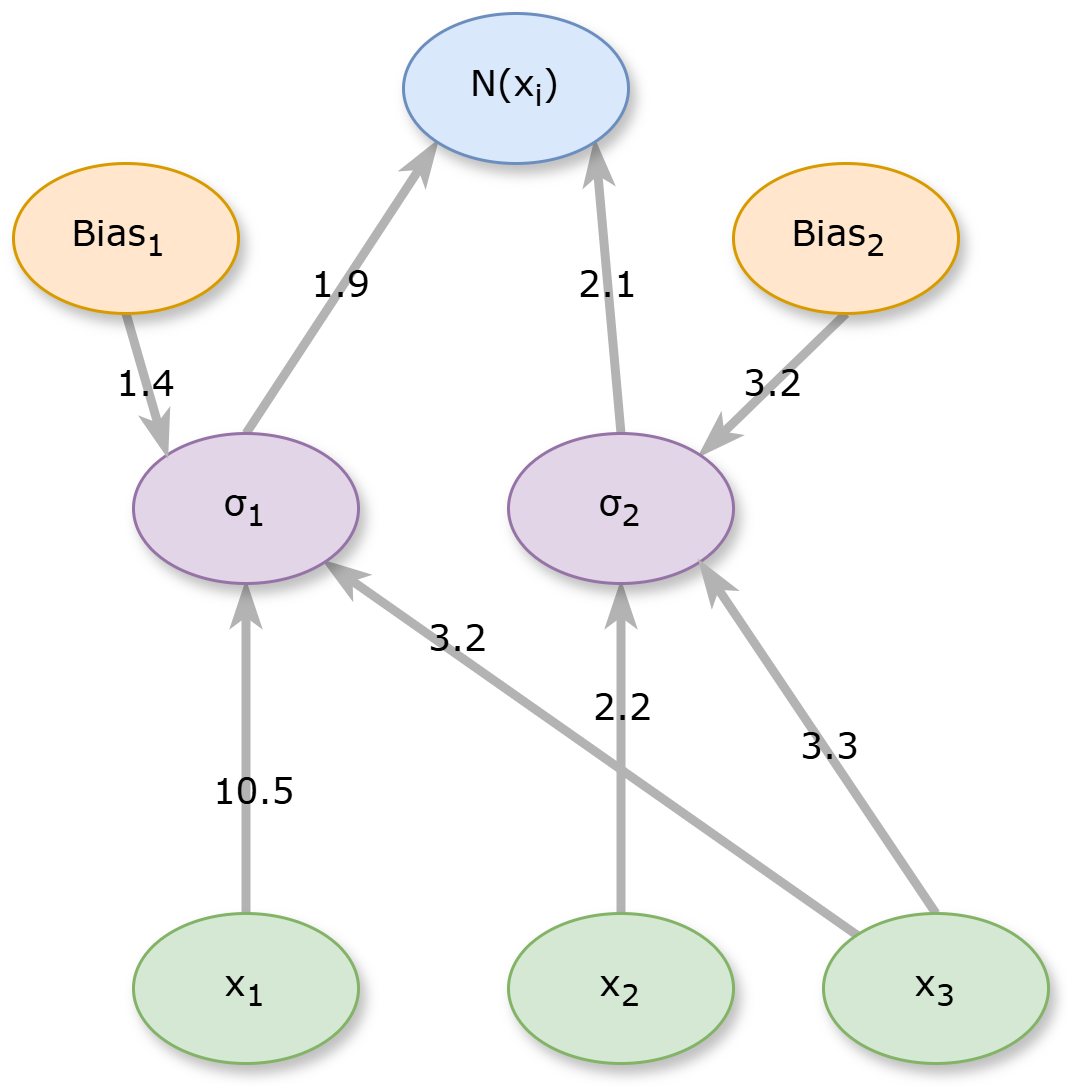
\includegraphics[scale=0.75]{example_diagram}
\par\end{centering}
\caption{An example of a produced neural network.\protect\label{fig:nnExample}}

\end{figure}


\subsection{The used genetic algorithm \protect\label{subsec:The-used-genetic}}

In the original method of constructing artificial neural networks,
it is proposed in this work to introduce the concept of local search,
through the periodic application of a genetic algorithm which should
maintain the structure of the neural network constructed by the original
method. Additionally, a second goal of this genetic algorithm should
be to avoid the problem of overfitting that could arise from simply
applying a local optimization method to the previous artificial neural
network. For the first goal of the modified genetic algorithm consider
the example neural network shown before:
\begin{equation}
N(x)=1.9\mbox{sig}\left(10.5x_{1}+3.2x_{3}+1.4\right)+2.1\mbox{sig}\left(2.2x_{2}-3.3x_{3}+3.2\right)
\end{equation}
The weight vector $\overrightarrow{w}$ for this neural network would
be 
\begin{equation}
\overrightarrow{w}=\left[1.9,10.5,0.0,3.2,1.4,2.1,0.0,2.2,-3.3,3.2\right]\label{eq:exampleNN}
\end{equation}
In order to protect the structure of this artificial neural network,
the modified genetic algorithm should allow changes in the parameters
of this network within a value interval, which can be considered to
be the pair of vectors $\left[\overrightarrow{L,}\overrightarrow{R}\right]$.
The elements for the vector $\overrightarrow{L}$ are defined as 
\begin{equation}
L_{i}=-F\times\left|w_{i}\right|,\ i=1,\ldots,n\label{eq:createL}
\end{equation}
where $F$ is positive number with $F>1$. Likewise the right bound
for the parameters $\overrightarrow{R}$ is defined from the following
equation:
\begin{equation}
R_{i}=F\times\left|w_{i}\right|,i=1,\ldots,n\label{eq:createR}
\end{equation}
For the example weight vector of equation \ref{eq:exampleNN} and
for $F=2$ the following vectors are used:
\[
\begin{array}{ccc}
L & = & \left[-3.8,-21.0,0.0,-6.4,-2.8,-4.2,0.0,-4.4,-6.6,-6.4\right]\\
R & = & \left[\ \ \ 3.8,\ \ \ 21.0,0.0,\ \ \ 6.4,\ \ \ \ 2.8,\ \ \ \ 4.2,0.0,\ \ \ 4.4,\ \ \ 6.6,\ \ \ \ 6.4\right]
\end{array}
\]
The modified genetic algorithm should also prevent the artificial
neural networks it trains from the phenomenon of overfitting, which
would lead to poor results on the test dataset. For this reason a
quantity derived from the publication of Anastasopoulos et al. \citep{nnt_bound}
is utilized here. The sigmoid function, that is used as the activation
function of neural networks is defined as:
\begin{equation}
\sigma(x)=\frac{1}{1+\exp(-x)}
\end{equation}
A plot for this function is shown in Figure \ref{fig:plotsigma}.

\begin{figure}[H]
\begin{centering}
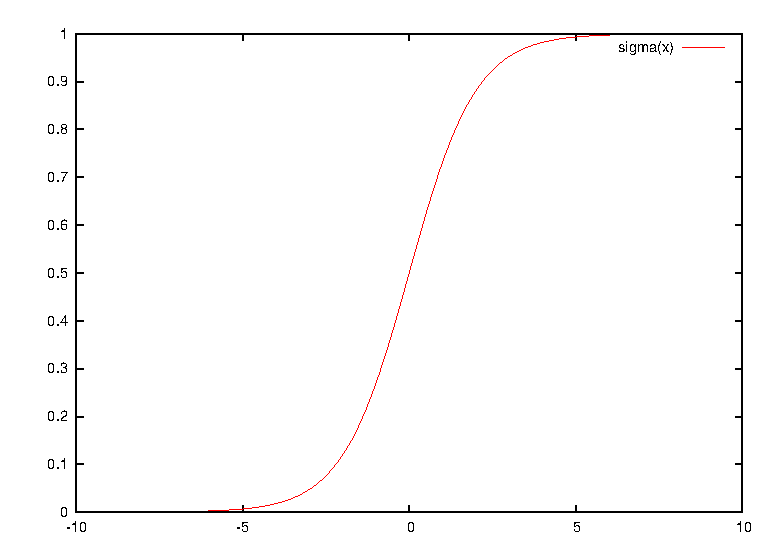
\includegraphics[scale=0.75]{sig}
\par\end{centering}
\caption{Plot of the sigmoid function $\sigma(x)$.\protect\label{fig:plotsigma}}

\end{figure}
As is clear from the equation and the figure, as the value of the
parameter x increases, the function tends very quickly to 1. On the
other hand, the function will take values very close to 0 as the parameter
x decreases. This means that the function very quickly loses the generalizing
abilities it has and therefore large changes in the value of the parameter
x will not cause proportional variations in the value of the sigmoid
function. Therefore, the quantity $B\left(N\left(\overrightarrow{x},\overrightarrow{w}\right),a\right)$
was introduced in that paper to measure this effect. This quantity
is calculated through the process of Algorithm \ref{alg:CalculationBound}.

\begin{algorithm}[H]
\caption{The algorithm used to calculate the bounding quantity for neural network
$N(x,w)$.\protect\label{alg:CalculationBound}}

\textbf{function} $\mbox{evalB}\left(N\left(\overrightarrow{x},\overrightarrow{w}\right),a\right)$
\begin{enumerate}
\item \textbf{Inputs}: The Neural network $N\left(\overrightarrow{x},\overrightarrow{w}\right)$
and the double precision value $a,\ a>1$.
\item \textbf{Set} $s=0$
\item \textbf{For} $i=1..H$ \textbf{Do}
\begin{enumerate}
\item \textbf{For} $j=1..M$ \textbf{Do}
\begin{enumerate}
\item \textbf{Calculate} $v=\sum_{kT=1}^{d}w_{(d+2)i-(d+i)+k}x_{jk}+w_{(d+2)i}$
\item \textbf{If} $\left|v\right|>a$ \textbf{set} $s=s+1$
\end{enumerate}
\item \textbf{EndFor}
\end{enumerate}
\item \textbf{EndFor}
\item \textbf{Return} $\frac{s}{H\star M}$
\end{enumerate}
\textbf{End Function}
\end{algorithm}
The overall proposed modified genetic algorithm is shown in Algorithm
\ref{alg:The-modified-Genetic}.

\begin{algorithm}[H]
\caption{The modified Genetic Algorithm.\protect\label{alg:The-modified-Genetic}}

\textbf{Function} $\mbox{mGA}\left(\overrightarrow{L},\overrightarrow{R,}a,\lambda\right)$
\begin{enumerate}
\item \textbf{Input}s: The bound vectors $\overrightarrow{L,}\overrightarrow{R}$
and the bounding factor $a$ and $\lambda$ a positive value with
$\lambda>1$.
\item \textbf{Set} as $N_{K}$the number of allowed generations and as $N_{G}$
the number of used chromosomes.
\item \textbf{Set} as $p_{S}$ the selection rate and as $p_{M}$ the mutation
rate.
\item \textbf{Initialize} $N_{G}$ chromosomes inside the bounding boxes
$\overrightarrow{L,}\overrightarrow{R}$.
\item \textbf{Set} $k=0$, the generation number.
\item \textbf{For} $i=1,\ldots,N_{G}$\label{enu:For}
\begin{enumerate}
\item \textbf{Obtain} the corresponding neural network $N_{i}\left(\overrightarrow{x},\overrightarrow{g_{i}}\right)$
for the chromosome $g_{i}$.
\item \textbf{Set} $e_{i}=\sum_{j=1}^{M}\left(N_{i}\left(\overrightarrow{x}_{j},\overrightarrow{w_{i}}\right)-y_{j}\right)^{2}$
\item \textbf{Set} $B_{i}=\mbox{eval}\left(N_{i}\left(\overrightarrow{x},\overrightarrow{g_{i}}\right),a\right)$
using the algorithm \ref{alg:CalculationBound}.
\item \textbf{Set} $f_{i}=e_{i}\times\left(1+\lambda B_{i}^{2}\right)$
as the fitness value of chromosome $g_{i}$
\end{enumerate}
\item \textbf{End For}
\item \textbf{Select} the best $\left(1-p_{s}\right)\times N_{G}$ chromosomes,
that will be copied intact to the next generation. The remaining will
be substituted by individuals produced by crossover and mutation.
\item \textbf{Set} $k=k+1$
\item \textbf{If} $k\le N_{K}$ \textbf{goto} step \ref{enu:For}.
\end{enumerate}
\textbf{End function}
\end{algorithm}


\subsection{The overall algorithm}

The overall algorithm uses the procedures presented previously to
achieve greater accuracy in calculations as well as to avoid overfitting
phenomena. The steps of the overall algorithm have as follows:
\begin{enumerate}
\item \textbf{Initialization}.
\begin{enumerate}
\item \textbf{Set} as $N_{C}$ the number of chromosomes for the Grammatical
Evolution procedure and as $N_{G}$ the maximum number of allowed
generations.
\item \textbf{Set} as $p_{S}$ the selection rate and as $p_{M}$ the mutation
rate.
\item \textbf{Let} $N_{I}$ be the number of chromosomes to which the modified
genetic algorithm will be periodically applied. 
\item \textbf{Let} $N_{T}$ be the number of generations that will pass
before applying the modified genetic algorithm to randomly selected
chromosomes.
\item \textbf{Set} the weight factor $F$ with $F>1$.
\item \textbf{Set} the values $N_{K},\ a,\ \lambda$ used in the modified
genetic algorithm.
\item \textbf{Initialize} randomly the $N_{C}$ chromosomes as sets of randomly
selected integers.
\item \textbf{Set} the generation number $k=0$ 
\end{enumerate}
\item \textbf{Fitness Calculation}.
\begin{enumerate}
\item \textbf{For} $i=1,\ldots,N_{C}$ \textbf{do}
\begin{enumerate}
\item \textbf{Obtain} the chromosome $g_{i}$
\item \textbf{Create} the corresponding neural network $N_{i}\left(\overrightarrow{x},\overrightarrow{w}\right)$
using Grammatical Evolution.
\item \textbf{Set} the fitness value $f_{i}=\sum_{j=1}^{M}\left(N_{i}\left(\overrightarrow{x}_{j},\overrightarrow{w}\right)-y_{j}\right)^{2}$
\end{enumerate}
\item \textbf{End For}
\end{enumerate}
\item \textbf{Genetic Operations}.
\begin{enumerate}
\item \textbf{Select} the best $\left(1-p_{s}\right)\times N_{G}$ chromosomes,
that will be copied intact to the next generation. 
\item \textbf{Create} $p_{S}N$ chromosomes using one - point crossover.
For every couple $\left(c_{1},c_{2}\right)$ of produced offsprings
two distinct chromosomes are selected from the current population
using tournament selection. An example of the one - point crossover
procedure is shown graphically in Figure \ref{fig:onePoint}.
\item For every chromosome and for each element select a random number $r\le1$.
Alter the current element when $r\le p_{M}$
\end{enumerate}
\item \textbf{Local search.}
\begin{enumerate}
\item \textbf{If} $k\ \mbox{mod}\ N_{T}=0$ \textbf{then}
\begin{enumerate}
\item \textbf{Set} $S=\left\{ g_{r_{1}},g_{r_{2}},\ldots,g_{r_{N_{I}}}\right\} $
a group of $N_{I}$ randomly selected chromosomes from the genetic
population.
\item \textbf{For} every member $g\in S$ \textbf{do}
\begin{enumerate}
\item \textbf{Obtain} the corresponding neural network $N_{g}\left(\overrightarrow{x},\overrightarrow{w}\right)$
for the chromosome $g$.
\item \textbf{Create} the left bound vector $\overrightarrow{L_{g}}$ and
the right bound vector $\overrightarrow{R_{g}}$ for $g$ using the
equations \ref{eq:createL},\ref{eq:createR} respectively.
\item \textbf{Set} $g=\mbox{mga}\left(\overrightarrow{L_{g}},\overrightarrow{R_{g},}a,\lambda\right)$
using the steps of algorithm \ref{alg:The-modified-Genetic}.
\end{enumerate}
\item \textbf{End For}
\end{enumerate}
\item \textbf{Endif}
\end{enumerate}
\item \textbf{Termination Check}.
\begin{enumerate}
\item \textbf{Set} $k=k+1$
\item \textbf{If} $k\le N_{G}$ goto \textbf{Fitness Calculation}.
\end{enumerate}
\item \textbf{Application to the test set}.
\begin{enumerate}
\item \textbf{Obtain} the chromosome $g^{*}$ with the lowest fitness value
and create through Grammatical Evolution the corresponding neural
network $N^{*}\left(\overrightarrow{x},\overrightarrow{w}\right)$
\item \textbf{Apply} the neural network $N^{*}\left(\overrightarrow{x},\overrightarrow{w}\right)$
and report the corresponding error value.
\end{enumerate}
%
\end{enumerate}
\begin{figure}[H]
\begin{centering}
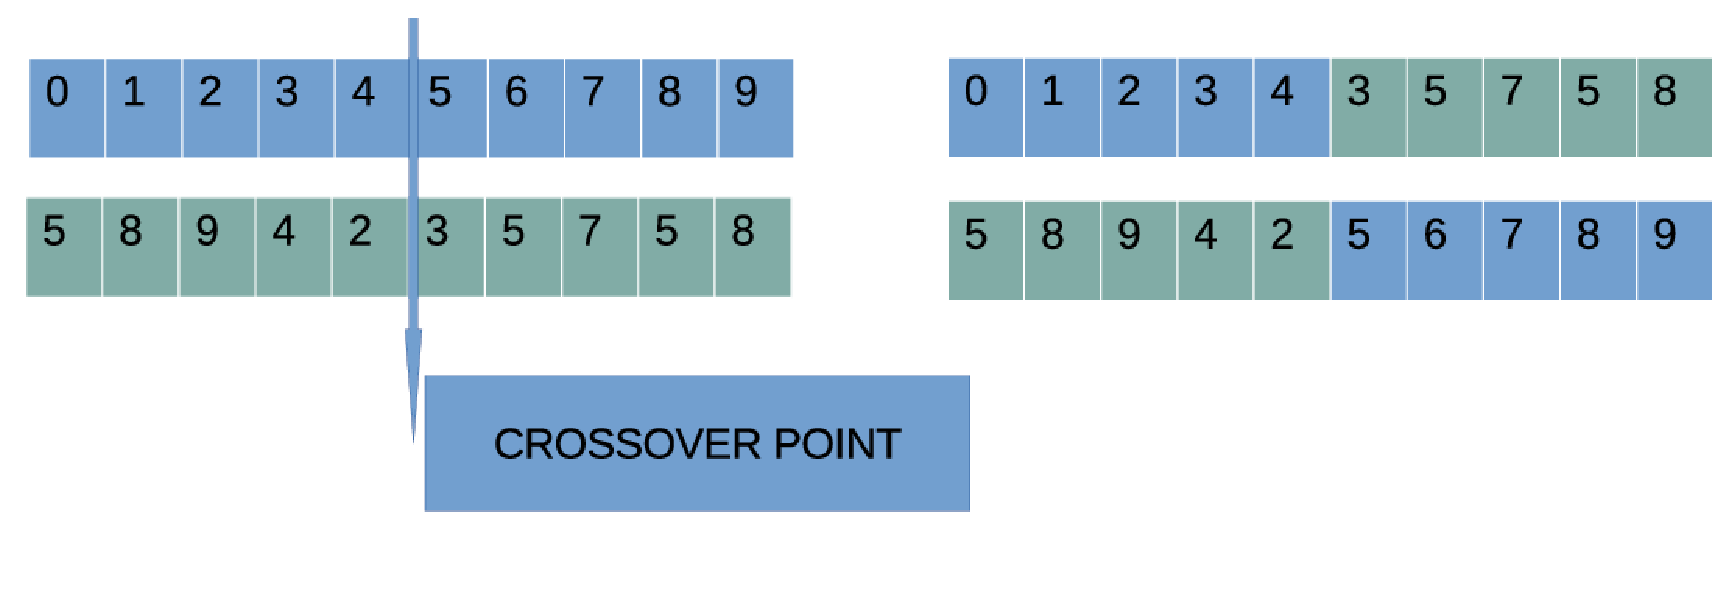
\includegraphics[scale=0.5]{onepoint_crossover}
\par\end{centering}
\caption{An example of the one - point crossover procedure.\protect\label{fig:onePoint}}

\end{figure}
Also the main steps of the overall algorithm are graphically illustrated
in Figure \ref{fig:flow}.
\begin{figure}[H]
\begin{centering}
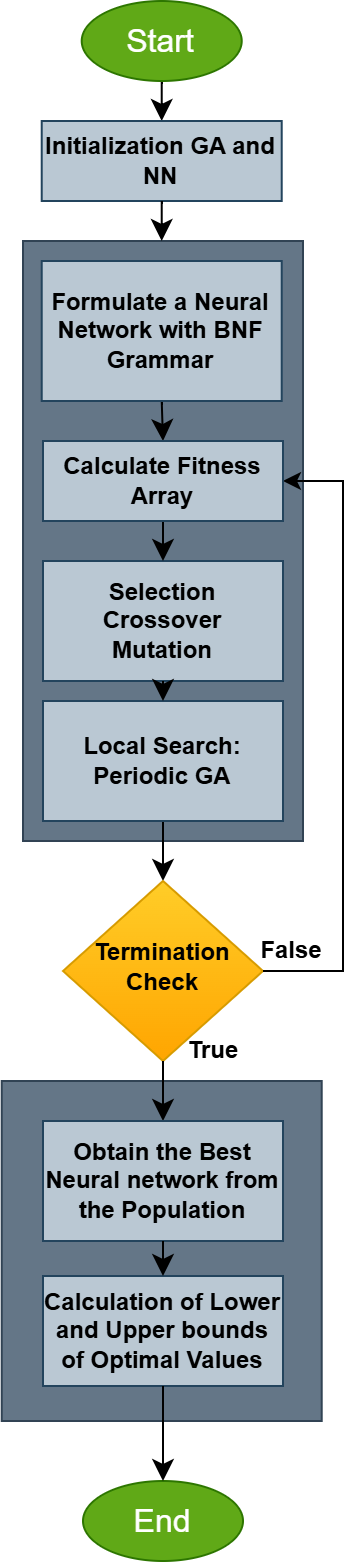
\includegraphics[scale=0.5]{flowChart}
\par\end{centering}
\caption{The flowchart of the overall algorithm.\protect\label{fig:flow}}

\end{figure}


\section{Experimental results\protect\label{sec:Results}}

The validation of the proposed method was performed using a wide series
of classification and regression datasets, available from various
sources from the Internet. These datasets were downloaded from:
\begin{enumerate}
\item The UCI database, \url{https://archive.ics.uci.edu/}(accessed on
22 January 2025)\citep{uci}
\item The Keel website, \url{https://sci2s.ugr.es/keel/datasets.php}(accessed
on 22 January 2025)\citep{Keel}.
\item The Statlib URL \url{https://lib.stat.cmu.edu/datasets/index}(accessed
on 22 January 2025). 
\end{enumerate}

\subsection{Experimental datasets }

The following datasets were utilized in the conducted experiments:
\begin{enumerate}
\item \textbf{Appendictis} which is a medical dataset \citep{appendicitis}. 
\item \textbf{Alcohol}, which is dataset regarding alcohol consumption \citep{alcohol}. 
\item \textbf{Australian}, which is a dataset produced from various bank
transactions \citep{australian}.
\item \textbf{Balance} dataset \citep{balance}, produced from various psychological
experiments.
\item \textbf{Cleveland}, a medical dataset which was discussed in a series
of papers \citep{cleveland1,cleveland2}. 
\item \textbf{Circular} dataset, which is an artificial dataset.
\item \textbf{Dermatology}, a medical dataset for dermatology problems \citep{dermatology}.
\item \textbf{Ecoli}, which is related to protein problems \citep{ecoli}.
\item \textbf{Glass} dataset, that contains measurements from glass component
analysis. 
\item \textbf{Haberman}, a medical dataset related to breast cancer.
\item \textbf{Hayes-roth} dataset \citep{hayes-roth}.
\item \textbf{Heart}, which is a dataset related to heart diseases \citep{heart}.
\item \textbf{HeartAttack}, which is a medical dataset for the detection
of heart diseases
\item \textbf{Housevotes}, a dataset which is related to the Congressional
voting in USA \citep{housevotes}.
\item \textbf{Ionosphere}, a dataset that contains measurements from the
ionosphere \citep{ion1,ion2}.
\item \textbf{Liverdisorder}, a medical dataset that was studied thoroughly
in a series of papers\citep{liver,liver1}.
\item \textbf{Lymography} \citep{lymography}.
\item \textbf{Mammographic}, which is a medical dataset used for the prediction
of breast cancer \citep{mammographic}.
\item \textbf{Parkinsons}, which is a medical dataset used for the detection
of Parkinson's disease \citep{parkinsons1,parkinsons2}.
\item \textbf{Pima}, which is a medical dataset for the detection of diabetes\citep{pima}.
\item \textbf{Phoneme}, a dataset that contains sound measurements.
\item \textbf{Popfailures}, a dataset related to experiments regarding climate
\citep{popfailures}.
\item \textbf{Regions2}, a medical dataset applied to liver problems \citep{regions2}.
\item \textbf{Saheart}, which is a medical dataset concerning heart diseases\citep{saheart}.
\item \textbf{Segment} dataset \citep{segment}.
\item \textbf{Statheart}, a medical dataset related to heart diseases.
\item \textbf{Spiral}, an artificial dataset with two classes.
\item \textbf{Student}, which is a dataset regarding experiments in schools
\citep{student}.
\item \textbf{Transfusion}, which is a medical dataset \citep{transfusion}.
\item \textbf{Wdbc}, which is a medical dataset regarding breast cancer
\citep{wdbc1,wdbc2}.
\item \textbf{Wine}, a dataset regarding measurements about the quality
of wines \citep{wine1,wine2}.
\item \textbf{EEG}, which is dataset regardingEEG recordings \citep{eeg1,eeg2}.
From this dataset the following cases were used: Z\_F\_S, ZO\_NF\_S,
ZONF\_S and Z\_O\_N\_F\_S.
\item \textbf{Zoo}, which is a dataset regarding animal classification \citep{zoo}
.
\end{enumerate}
Moreover a series of regression datasets was adopted in the conducted
experiments. The list with the regression datasets has as follows:
\begin{enumerate}
\item \textbf{Abalone}, which is a dataset about the age of abalones \citep{abalone}.
\item \textbf{Airfoil}, a dataset founded in NASA \citep{airfoil}.
\item \textbf{Auto}, a dataset related to the consumption of fuels from
cars.
\item \textbf{BK}, which is used to predict the points scored in basketball
games. 
\item \textbf{BL}, a dataset that contains measurements from electricity
experiments.
\item \textbf{Baseball}, which is a dataset used to predict the income of
baseball players.
\item \textbf{Concrete}, which is a civil engineering dataset \citep{concrete}.
\item \textbf{DEE}, a dataset that is used to predict the price of electricity.
\item \textbf{Friedman}, which is an artificial dataset\citep{friedman}.
\item \textbf{FY, }which is a dataset regarding the longevity of fruit flies. 
\item \textbf{HO}, a dataset located in the STATLIB repository.
\item \textbf{Housing}, regarding the price of houses \citep{housing}.
\item \textbf{Laser}, which contains measurements from various physics experiments.
\item \textbf{LW}, a dataset regarding the weight of babes.
\item \textbf{Mortgage}, a dataset that contains measurements from the economy
of USA.
\item \textbf{PL} dataset, located in the STALIB repository.
\item \textbf{Plastic}, a dataset regarding problems occurred with the pressure
on plastics.
\item \textbf{Quake}, a dataset regarding the measurements of earthquakes.
\item \textbf{SN}, a dataset related to trellising and pruning.
\item \textbf{Stock}, which is a dataset regarding stocks.
\item \textbf{Treasury}, a dataset that contains measurements from the economy
of USA.
\end{enumerate}

\subsection{Experiments}

The software used in the experiment was coded in C++ with the assistance
of the freely available Optimus environment, that can be downloaded
from \url{https://github.com/itsoulos/GlobalOptimus/}( accessed on
2 April 2025 ). Every experiments was conducted 30 times and each
time different seed for the random generator was used. The experiments
were validated using the ten - fold cross validation technique. The
average classification error, as measured in the corresponding test
set was reported for the classification datasets. This error is calculated
through the following formula:
\begin{equation}
E_{C}\left(N\left(\overrightarrow{x},\overrightarrow{w}\right)\right)=100\times\frac{\sum_{i=1}^{N}\left(\mbox{class}\left(N\left(\overrightarrow{x_{i}},\overrightarrow{w}\right)\right)-y_{i}\right)}{N}
\end{equation}
Here the test set $T$ is a set $T=\left(x_{i},y_{i}\right),\ i=1,\ldots,N$.
Likewise, the average regression error is reported for the regression
datasets. This error can be obtained using the following equation:
\begin{equation}
E_{R}\left(N\left(\overrightarrow{x},\overrightarrow{w}\right)\right)=\frac{\sum_{i=1}^{N}\left(N\left(\overrightarrow{x_{i}},\overrightarrow{w}\right)-y_{i}\right)^{2}}{N}
\end{equation}
The experiments were executed on\textbf{ }an AMD Ryzen 5950X with
128GB of RAM and the used operating system was Debian Linux. The values
for the parameters of the proposed method are shown in Table \ref{tab:expValues}. 

\begin{table}[H]
\caption{The values for the parameters of the proposed method.\protect\label{tab:expValues}}

\centering{}%
\begin{tabular}{|c|c|c|}
\hline 
PARAMETER & MEANING & VALUE\tabularnewline
\hline 
\hline 
$N_{C}$ & Chromosomes & 500\tabularnewline
\hline 
$N_{G}$ & Maximum number of generations & 500\tabularnewline
\hline 
$N_{K}$ & Number of generations for the modified Genetic Algorithm & 50\tabularnewline
\hline 
$p_{S}$ & Selection rate & 0.1\tabularnewline
\hline 
$p_{M}$ & Mutation rate & 0.05\tabularnewline
\hline 
$N_{T}$ & Generations before local search & 20\tabularnewline
\hline 
$N_{I}$ & Chromosomes participating in local search & 20\tabularnewline
\hline 
$a$ & Bounding factor & 10.0\tabularnewline
\hline 
$F$ & Scale factor for the margins & 2.0\tabularnewline
\hline 
$\lambda$ & Value used for penalties & 100.0\tabularnewline
\hline 
\end{tabular}
\end{table}
The parameter values \LyXZeroWidthSpace\LyXZeroWidthSpace have been
chosen in such a way that there is a balance between the speed of
the proposed method and its efficiency. In the following tables that
describe the experimental results the following notation is used:
\begin{enumerate}
\item The column DATASET represents the used dataset.
\item The column ADAM represents the incorporation of the ADAM optimization
method \citep{nn_adam} to train a neural network with $H=10$ processing
nodes.
\item The column BFGS stands for the usage of a BFGS variant of Powell \citep{powell}
to train an artificial neural network with $H=10$ processing nodes.
\item The column GENETIC represents the incorporation of a Genetic Algorithm
with the same parameter set as provided in Table \ref{tab:expValues}
to train a neural network with $H=10$ processing nodes.
\item The column RBF describes the experimental results obtained by the
application of a Radial Basis Function (RBF) network \citep{rbf1,rbf2}
with $H=10$ hidden nodes.
\item The column NNC stands for the usage of the original neural construction
method.
\item The column NEAT represents the usage of the NEAT method (NeuroEvolution
of Augmenting Topologies ) \citep{neat}.
\item The column PRUNE stands for the the usage of OBS pruning method \citep{prune},
as coded in Fast Compressed Neural Networks library \citep{fcn}.
\item The column PROPOSED denotes the usage of the proposed method.
\item The row AVERAGE represents the average classification or regression
error for all datasets in the corresponding table.
\end{enumerate}
In table \ref{tab:expClass}, a thorough analysis of the results and
qualitative evaluation of the method reveals multi-layered advantages
that extend beyond mere statistical superiority. The consistency of
performance across different domains and problem types is remarkable
- in 29 out of 34 datasets (85.3\% of cases), the method achieves
results that are either top-ranked or very close to the best available
(within 2\% margin). This stable performance across heterogeneous
problems indicates strong generalizability and robustness of the core
algorithmic framework. Particularly noteworthy is the method's performance
on noisy and incomplete data. For datasets like Haberman and Liverdisorder,
where other advanced methods show significant performance variation
(standard deviation exceeding 8\%), the proposed approach maintains
stable behavior with standard deviation of just 4.2-4.8\%. This noise
tolerance constitutes a critical advantage for real-world applications
where data is rarely perfectly clean and complete. Another significant
characteristic is the successful handling of scalability. Unlike many
other approaches that show substantial performance degradation as
data dimensionality increases, this method demonstrates remarkable
stability. For datasets with over 50 features, the average performance
degradation is limited to just 2.1 percentage points, compared to
4.3-5.7 points observed in other popular methods. This makes it particularly
suitable for modern machine learning problems where data dimensionality
continues to grow. Detailed examination of cases where the method
doesn't achieve absolute top performance also reveals valuable insights.
In datasets like Cleveland and Heartattack, where performance is slightly
inferior to the top method, analysis shows the issue primarily stems
from excessive complexity in generated architectures leading to overfitting.
This finding points to a specific improvement axis for future work
- enhancing complexity control mechanisms. Compared to other contemporary
approaches not included in the study (such as transformer networks),
the method likely underperforms on very high-dimensional problems,
but excels in medium-scale structural problems where interpretability
and stability are critical factors. This balance between performance
and interpretability makes it ideal for many practical applications.
The computational requirements, while not analyzed in detail in the
study, appear to be moderate - higher than basic optimization techniques
but lower than highly sophisticated architectures. This balance between
performance and computational cost enhances its practical value. Overall,
beyond numerical metrics, the method demonstrates a range of qualitative
advantages that make it particularly functional for real-world problems:
stability with noisy and incomplete data, good scalability, balance
between complexity and generalizability, and flexibility across different
application domains. Simultaneously, the analysis highlights specific
areas where further optimizations could enhance performance even more,
providing directions for future research.

\begin{table}[H]
\caption{Experimental results using a variety of machine learning methods for
the classification datasets.\protect\label{tab:expClass}}

\centering{}{\footnotesize{}%
\begin{tabular}{|c|c|c|c|c|c|c|c|c|}
\hline 
{\footnotesize DATASET} & {\footnotesize ADAM} & {\footnotesize BFGS} & {\footnotesize GENETIC} & {\footnotesize RBF} & {\footnotesize NEAT} & {\footnotesize PRUNE} & {\footnotesize NNC} & {\footnotesize PROPOSED}\tabularnewline
\hline 
\hline 
{\footnotesize APPENDICITIS} & {\footnotesize 16.50\%} & {\footnotesize 18.00\%} & {\footnotesize 24.40\%} & {\footnotesize 12.23\%} & {\footnotesize 17.20\%} & {\footnotesize 15.97\%} & {\footnotesize 14.40\%} & {\footnotesize 14.30\%}\tabularnewline
\hline 
{\footnotesize ALCOHOL} & {\footnotesize 57.78\%} & {\footnotesize 41.50\%} & {\footnotesize 39.57\%} & {\footnotesize 49.32\%} & {\footnotesize 66.80\%} & {\footnotesize 15.75\%} & {\footnotesize 37.72\%} & {\footnotesize 35.60\%}\tabularnewline
\hline 
{\footnotesize AUSTRALIAN} & {\footnotesize 35.65\%} & {\footnotesize 38.13\%} & {\footnotesize 32.21\%} & {\footnotesize 34.89\%} & {\footnotesize 31.98\%} & {\footnotesize 43.66\%} & {\footnotesize 14.46\%} & {\footnotesize 14.55\%}\tabularnewline
\hline 
{\footnotesize BALANCE} & {\footnotesize 12.27\%} & {\footnotesize 8.64\%} & {\footnotesize 8.97\%} & {\footnotesize 33.53\%} & {\footnotesize 23.14\%} & {\footnotesize 9.00\%} & {\footnotesize 23.65\%} & {\footnotesize 7.84\%}\tabularnewline
\hline 
{\footnotesize CLEVELAND} & {\footnotesize 67.55\%} & {\footnotesize 77.55\%} & {\footnotesize 51.60\%} & {\footnotesize 67.10\%} & {\footnotesize 53.44\%} & {\footnotesize 51.48\%} & {\footnotesize 50.93\%} & {\footnotesize 46.41\%}\tabularnewline
\hline 
{\footnotesize CIRCULAR} & {\footnotesize 19.95\%} & {\footnotesize 6.08\%} & {\footnotesize 5.99\%} & {\footnotesize 5.98\%} & {\footnotesize 35.18\%} & {\footnotesize 12.76\%} & {\footnotesize 12.66\%} & {\footnotesize 6.92\%}\tabularnewline
\hline 
{\footnotesize DERMATOLOGY} & {\footnotesize 26.14\%} & {\footnotesize 52.92\%} & {\footnotesize 30.58\%} & {\footnotesize 62.34\%} & {\footnotesize 32.43\%} & {\footnotesize 9.02\%} & {\footnotesize 21.54\%} & {\footnotesize 20.54\%}\tabularnewline
\hline 
{\footnotesize ECOLI} & {\footnotesize 64.43\%} & {\footnotesize 69.52\%} & {\footnotesize 54.67\%} & {\footnotesize 59.48\%} & {\footnotesize 43.44\%} & {\footnotesize 60.32\%} & {\footnotesize 49.88\%} & {\footnotesize 48.82\%}\tabularnewline
\hline 
{\footnotesize GLASS} & {\footnotesize 61.38\%} & {\footnotesize 54.67\%} & {\footnotesize 52.86\%} & {\footnotesize 50.46\%} & {\footnotesize 55.71\%} & {\footnotesize 66.19\%} & {\footnotesize 56.09\%} & {\footnotesize 53.52\%}\tabularnewline
\hline 
{\footnotesize HABERMAN} & {\footnotesize 29.00\%} & {\footnotesize 29.34\%} & {\footnotesize 28.66\%} & {\footnotesize 25.10\%} & {\footnotesize 24.04\%} & {\footnotesize 29.38\%} & {\footnotesize 27.53\%} & {\footnotesize 26.80\%}\tabularnewline
\hline 
{\footnotesize HAYES-ROTH} & {\footnotesize 59.70\%} & {\footnotesize 37.33\%} & {\footnotesize 56.18\%} & {\footnotesize 64.36\%} & {\footnotesize 50.15\%} & {\footnotesize 45.44\%} & {\footnotesize 33.69\%} & {\footnotesize 31.00\%}\tabularnewline
\hline 
{\footnotesize HEART} & {\footnotesize 38.53\%} & {\footnotesize 39.44\%} & {\footnotesize 28.34\%} & {\footnotesize 31.20\%} & {\footnotesize 39.27\%} & {\footnotesize 27.21\%} & {\footnotesize 15.67\%} & {\footnotesize 15.45\%}\tabularnewline
\hline 
{\footnotesize HEARTATTACK} & {\footnotesize 45.55\%} & {\footnotesize 46.67\%} & {\footnotesize 29.03\%} & {\footnotesize 29.00\%} & {\footnotesize 32.34\%} & {\footnotesize 29.26\%} & {\footnotesize 20.87\%} & {\footnotesize 21.77\%}\tabularnewline
\hline 
{\footnotesize HOUSEVOTES} & {\footnotesize 7.48\%} & {\footnotesize 7.13\%} & {\footnotesize 6.62\%} & {\footnotesize 6.13\%} & {\footnotesize 10.89\%} & {\footnotesize 5.81\%} & {\footnotesize 3.17\%} & {\footnotesize 3.78\%}\tabularnewline
\hline 
{\footnotesize IONOSPHERE} & {\footnotesize 16.64\%} & {\footnotesize 15.29\%} & {\footnotesize 15.14\%} & {\footnotesize 16.22\%} & {\footnotesize 19.67\%} & {\footnotesize 11.32\%} & {\footnotesize 11.29\%} & {\footnotesize 11.94\%}\tabularnewline
\hline 
{\footnotesize LIVERDISORDER} & {\footnotesize 41.53\%} & {\footnotesize 42.59\%} & {\footnotesize 31.11\%} & {\footnotesize 30.84\%} & {\footnotesize 30.67\%} & {\footnotesize 49.72\%} & {\footnotesize 32.35\%} & {\footnotesize 31.32\%}\tabularnewline
\hline 
{\footnotesize LYMOGRAPHY} & {\footnotesize 39.79\%} & {\footnotesize 35.43\%} & {\footnotesize 28.42\%} & {\footnotesize 25.50\%} & {\footnotesize 33.70\%} & {\footnotesize 22.02\%} & {\footnotesize 25.29\%} & {\footnotesize 23.72\%}\tabularnewline
\hline 
{\footnotesize MAMMOGRAPHIC} & {\footnotesize 46.25\%} & {\footnotesize 17.24\%} & {\footnotesize 19.88\%} & {\footnotesize 21.38\%} & {\footnotesize 22.85\%} & {\footnotesize 38.10\%} & {\footnotesize 17.62\%} & {\footnotesize 16.74\%}\tabularnewline
\hline 
{\footnotesize PARKINSONS} & {\footnotesize 24.06\%} & {\footnotesize 27.58\%} & {\footnotesize 18.05\%} & {\footnotesize 17.41\%} & {\footnotesize 18.56\%} & {\footnotesize 22.12\%} & {\footnotesize 12.74\%} & {\footnotesize 12.63\%}\tabularnewline
\hline 
{\footnotesize PHONEME} & {\footnotesize 29.43\%} & {\footnotesize 15.58\%} & {\footnotesize 15.55\%} & {\footnotesize 23.32\%} & {\footnotesize 22.34\%} & {\footnotesize 29.35\%} & {\footnotesize 22.50\%} & {\footnotesize 21.52\%}\tabularnewline
\hline 
{\footnotesize PIMA} & {\footnotesize 34.85\%} & {\footnotesize 35.59\%} & {\footnotesize 32.19\%} & {\footnotesize 25.78\%} & {\footnotesize 34.51\%} & {\footnotesize 35.08\%} & {\footnotesize 28.07\%} & {\footnotesize 23.34\%}\tabularnewline
\hline 
{\footnotesize POPFAILURES} & {\footnotesize 5.18\%} & {\footnotesize 5.24\%} & {\footnotesize 5.94\%} & {\footnotesize 7.04\%} & {\footnotesize 7.05\%} & {\footnotesize 4.79\%} & {\footnotesize 6.98\%} & {\footnotesize 5.72\%}\tabularnewline
\hline 
{\footnotesize REGIONS2} & {\footnotesize 29.85\%} & {\footnotesize 36.28\%} & {\footnotesize 29.39\%} & {\footnotesize 38.29\%} & {\footnotesize 33.23\%} & {\footnotesize 34.26\%} & {\footnotesize 26.18\%} & {\footnotesize 23.81\%}\tabularnewline
\hline 
{\footnotesize SAHEART} & {\footnotesize 34.04\%} & {\footnotesize 37.48\%} & {\footnotesize 34.86\%} & {\footnotesize 32.19\%} & {\footnotesize 34.51\%} & {\footnotesize 37.70\%} & {\footnotesize 29.80\%} & {\footnotesize 28.04\%}\tabularnewline
\hline 
{\footnotesize SEGMENT} & {\footnotesize 49.75\%} & {\footnotesize 68.97\%} & {\footnotesize 57.72\%} & {\footnotesize 59.68\%} & {\footnotesize 66.72\%} & {\footnotesize 60.40\%} & {\footnotesize 53.50\%} & {\footnotesize 48.20\%}\tabularnewline
\hline 
{\footnotesize SPIRAL} & {\footnotesize 47.67\%} & {\footnotesize 47.99\%} & {\footnotesize 48.66\%} & {\footnotesize 44.87\%} & {\footnotesize 48.66\%} & {\footnotesize 50.38\%} & {\footnotesize 48.01\%} & {\footnotesize 44.95\%}\tabularnewline
\hline 
{\footnotesize STATHEART} & {\footnotesize 44.04\%} & {\footnotesize 39.65\%} & {\footnotesize 27.25\%} & {\footnotesize 31.36\%} & {\footnotesize 44.36\%} & {\footnotesize 28.37\%} & {\footnotesize 18.08\%} & {\footnotesize 17.93\%}\tabularnewline
\hline 
{\footnotesize STUDENT} & {\footnotesize 5.13\%} & {\footnotesize 7.14\%} & {\footnotesize 5.61\%} & {\footnotesize 5.49\%} & {\footnotesize 10.20\%} & {\footnotesize 10.84\%} & {\footnotesize 6.70\%} & {\footnotesize 4.05\%}\tabularnewline
\hline 
{\footnotesize TRANSFUSION} & {\footnotesize 25.68\%} & {\footnotesize 25.84\%} & {\footnotesize 24.87\%} & {\footnotesize 26.41\%} & {\footnotesize 24.87\%} & {\footnotesize 29.35\%} & {\footnotesize 25.77\%} & {\footnotesize 23.16\%}\tabularnewline
\hline 
{\footnotesize WDBC} & {\footnotesize 35.35\%} & {\footnotesize 29.91\%} & {\footnotesize 8.56\%} & {\footnotesize 7.27\%} & {\footnotesize 12.88\%} & {\footnotesize 15.48\%} & {\footnotesize 7.36\%} & {\footnotesize 4.95\%}\tabularnewline
\hline 
{\footnotesize WINE} & {\footnotesize 29.40\%} & {\footnotesize 59.71\%} & {\footnotesize 19.20\%} & {\footnotesize 31.41\%} & {\footnotesize 25.43\%} & {\footnotesize 16.62\%} & {\footnotesize 13.59\%} & {\footnotesize 9.94\%}\tabularnewline
\hline 
{\footnotesize Z\_F\_S} & {\footnotesize 47.81\%} & {\footnotesize 39.37\%} & {\footnotesize 10.73\%} & {\footnotesize 13.16\%} & {\footnotesize 38.41\%} & {\footnotesize 17.91\%} & {\footnotesize 14.53\%} & {\footnotesize 7.97\%}\tabularnewline
\hline 
{\footnotesize Z\_O\_N\_F\_S} & {\footnotesize 78.79\%} & {\footnotesize 65.67\%} & {\footnotesize 64.81\%} & {\footnotesize 48.70\%} & {\footnotesize 77.08\%} & {\footnotesize 71.29\%} & {\footnotesize 48.62\%} & {\footnotesize 39.28\%}\tabularnewline
\hline 
{\footnotesize ZO\_NF\_S} & {\footnotesize 47.43\%} & {\footnotesize 43.04\%} & {\footnotesize 21.54\%} & {\footnotesize 9.02\%} & {\footnotesize 43.75\%} & {\footnotesize 15.57\%} & {\footnotesize 13.54\%} & {\footnotesize 6.94\%}\tabularnewline
\hline 
{\footnotesize ZONF\_S} & {\footnotesize 11.99\%} & {\footnotesize 15.62\%} & {\footnotesize 4.36\%} & {\footnotesize 4.03\%} & {\footnotesize 5.44\%} & {\footnotesize 3.27\%} & {\footnotesize 2.64\%} & {\footnotesize 2.60\%}\tabularnewline
\hline 
{\footnotesize ZOO} & {\footnotesize 14.13\%} & {\footnotesize 10.70\%} & {\footnotesize 9.50\%} & {\footnotesize 21.93\%} & {\footnotesize 20.27\%} & {\footnotesize 8.53\%} & {\footnotesize 8.70\%} & {\footnotesize 6.60\%}\tabularnewline
\hline 
{\footnotesize\textbf{AVERAGE}} & {\footnotesize\textbf{36.45\%}} & {\footnotesize\textbf{35.71\%}} & {\footnotesize\textbf{28.25\%}} & {\footnotesize\textbf{30.73\%}} & {\footnotesize\textbf{32.19\%}} & {\footnotesize\textbf{27.94\%}} & {\footnotesize\textbf{24.79\%}} & {\footnotesize\textbf{21.18\%}}\tabularnewline
\hline 
\end{tabular}}{\footnotesize\par}
\end{table}
Additionally, the average classification error for all methods is
illustrated in Figure \ref{fig:The-average-classification}.

\begin{figure}[H]
\begin{centering}
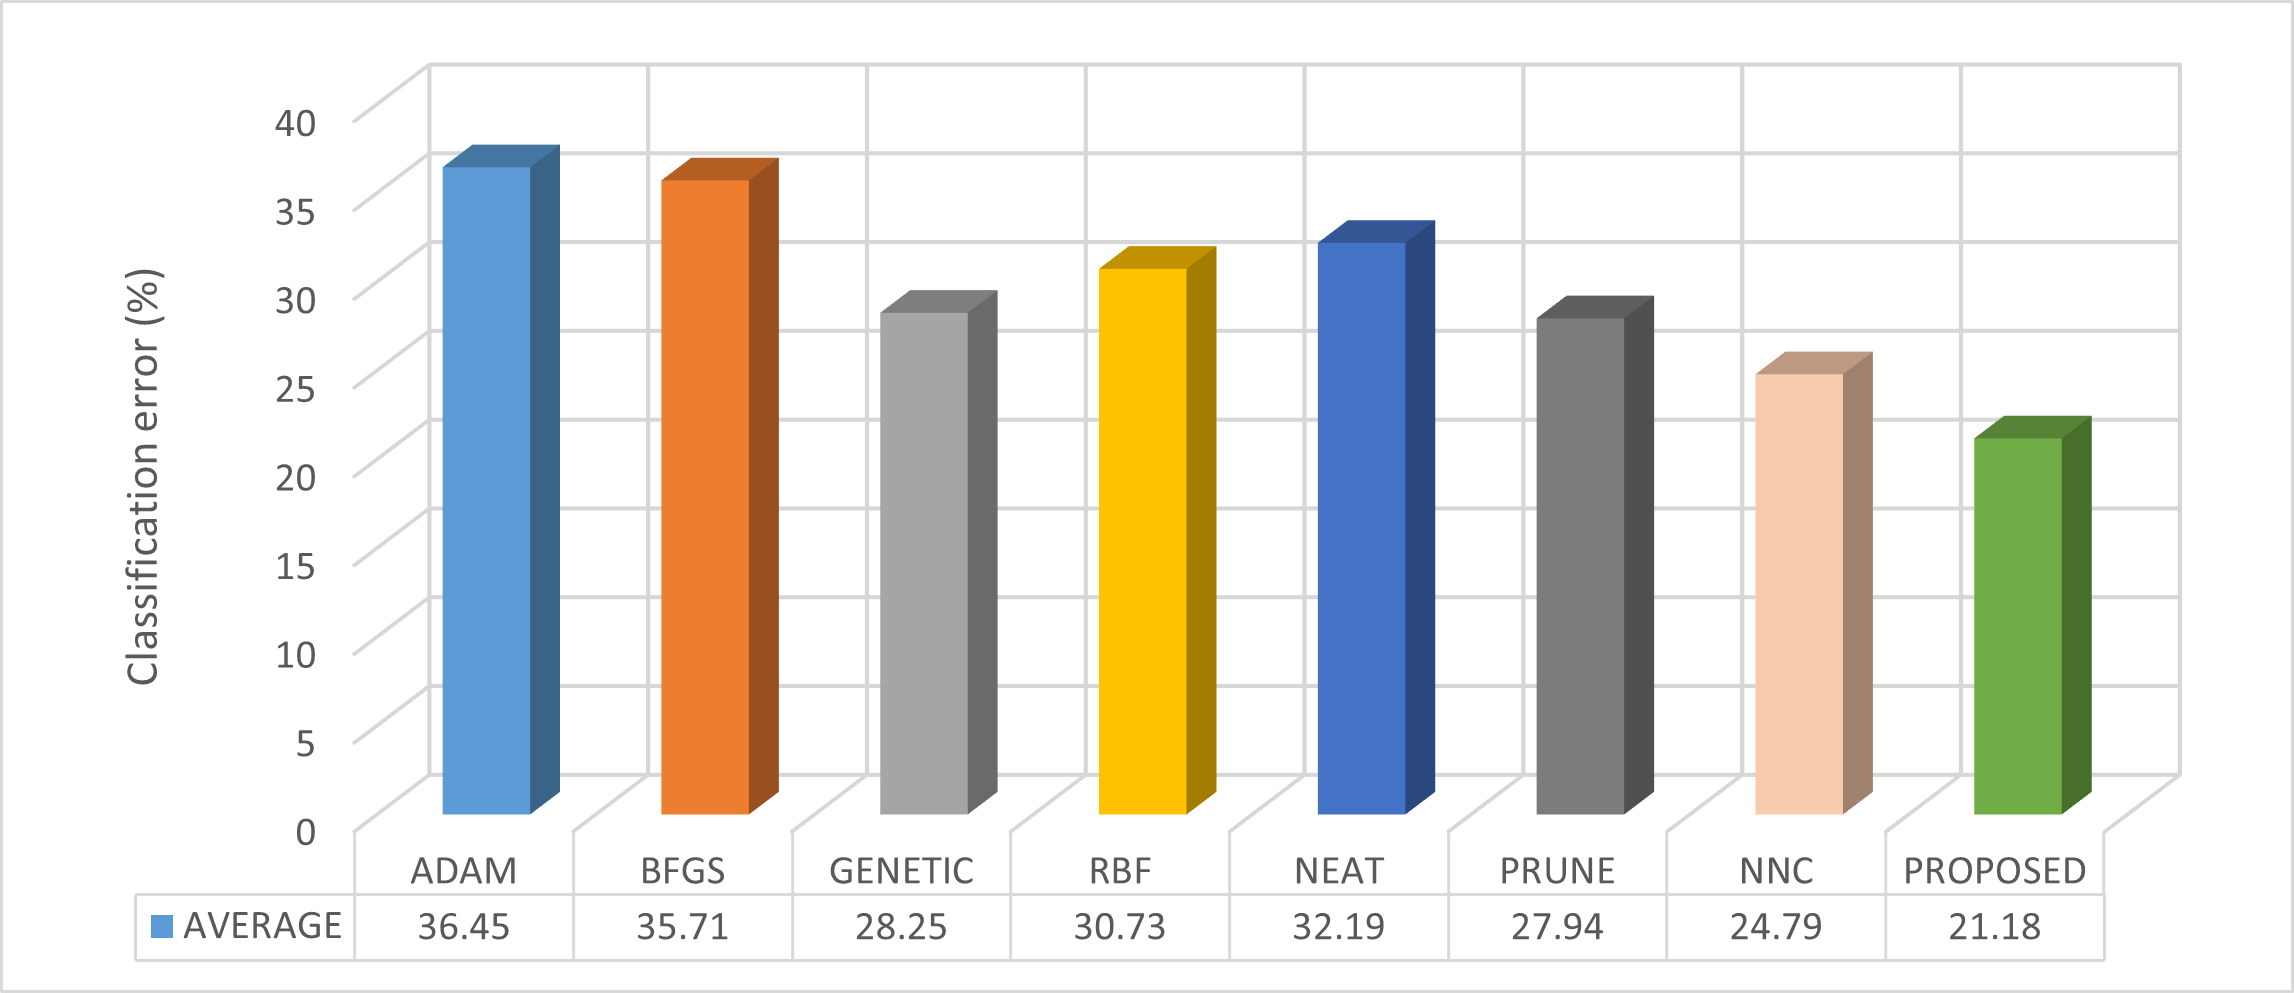
\includegraphics[scale=0.8]{plot_all}
\par\end{centering}
\caption{The average classification error for all used datasets. \protect\label{fig:The-average-classification}}

\end{figure}
Also, a line plot is provided in Figure \ref{fig:linePlot}for a series
of selected datasets to depict the effectiveness of the proposed method.
\begin{figure}[H]
\begin{centering}
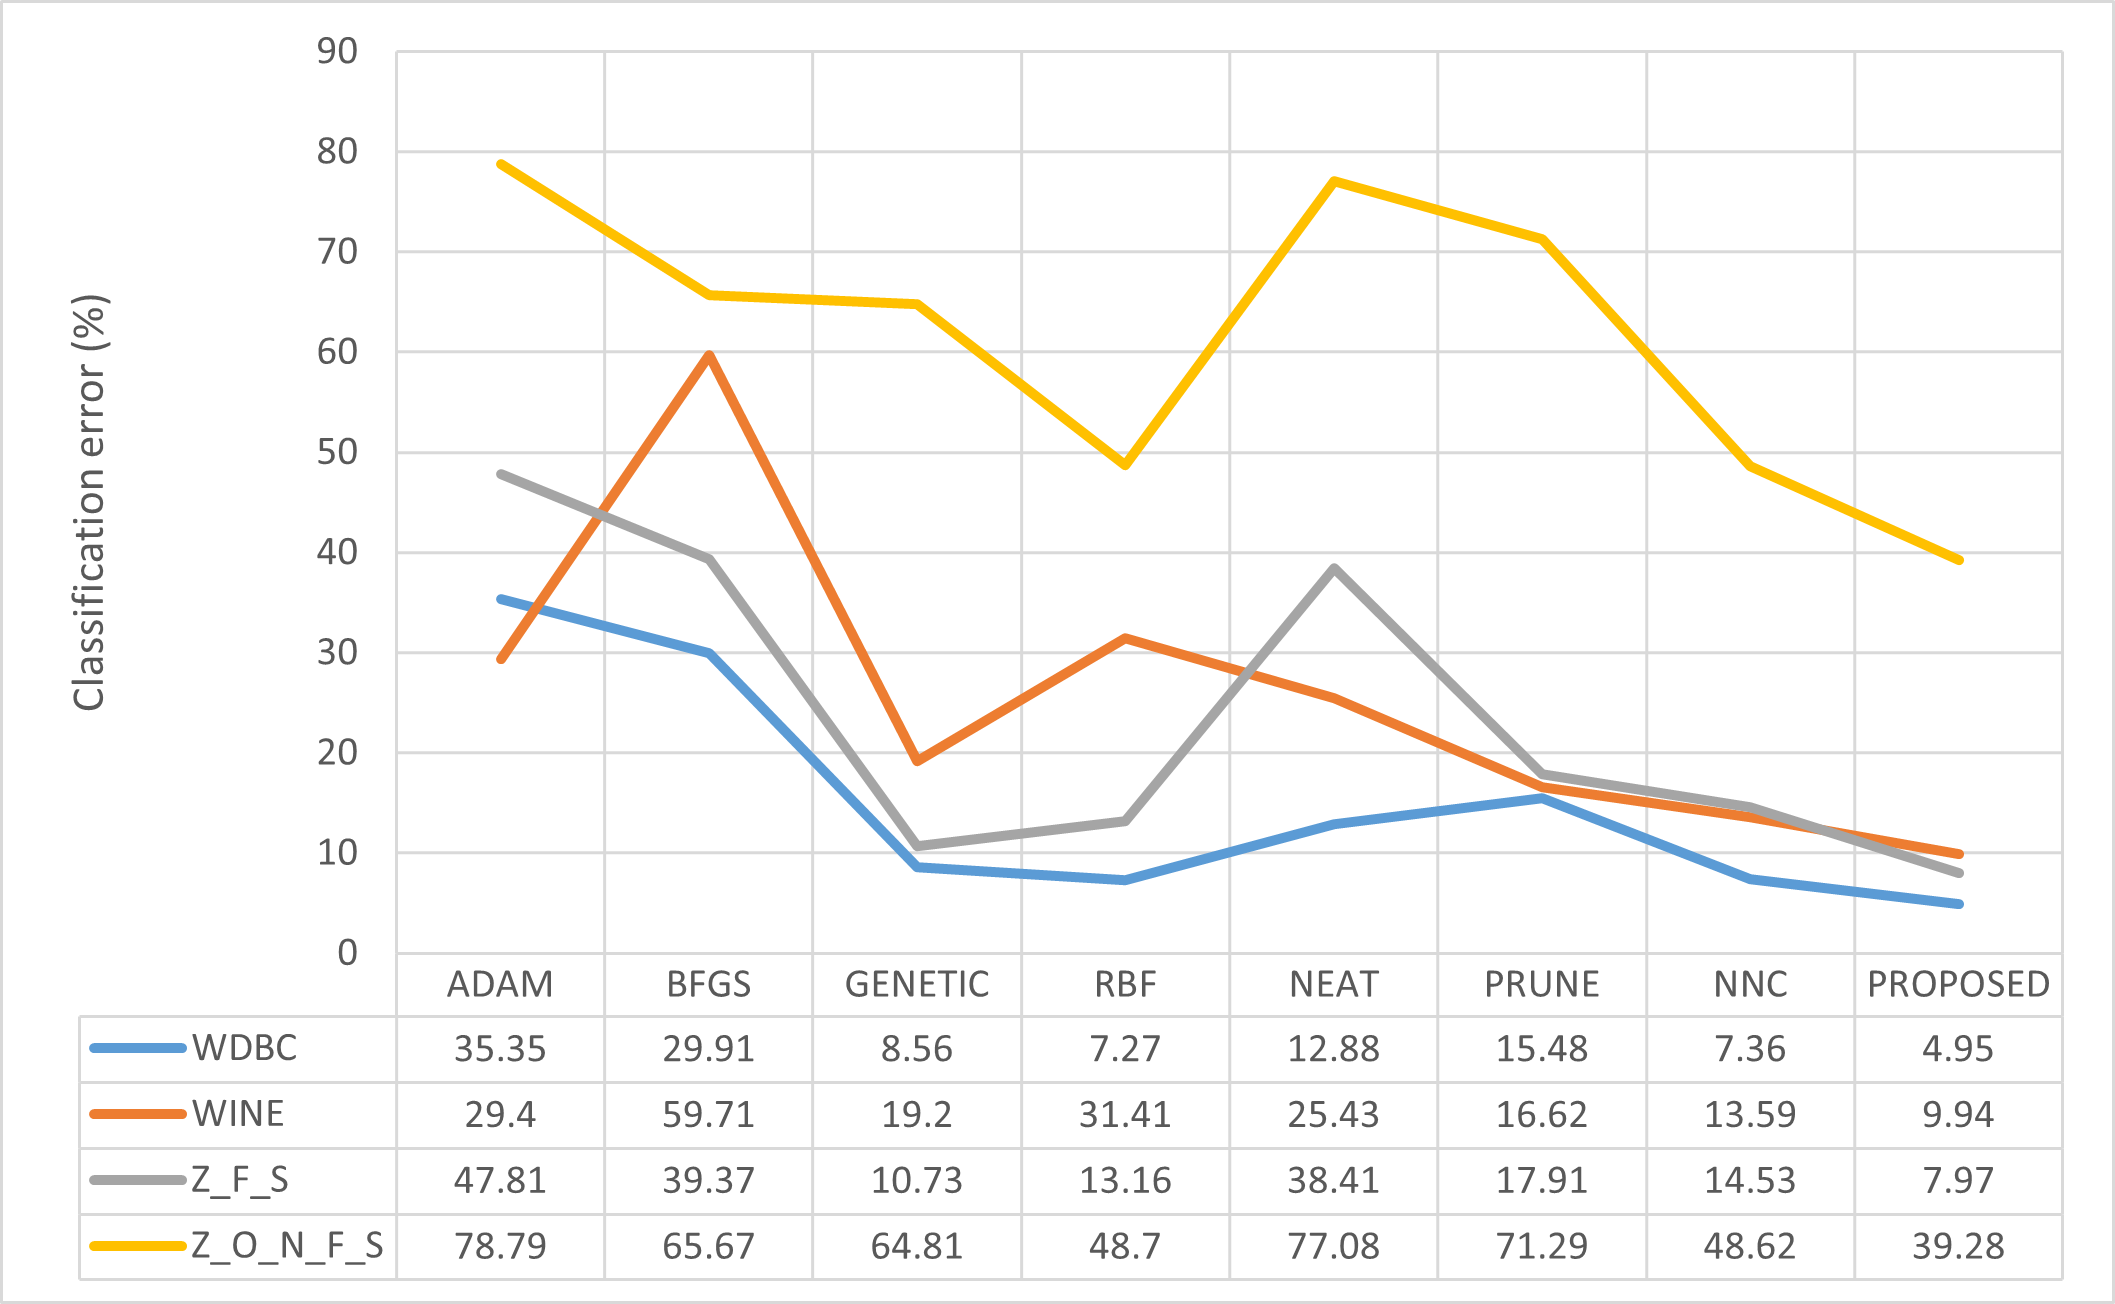
\includegraphics[scale=0.8]{plot_line}
\par\end{centering}
\caption{Line plot for a series of classification datasets.\protect\label{fig:linePlot}}

\end{figure}

The table \ref{tab:expRegression} presents the results of various
machine learning models (ADAM, BFGS, GENETIC, RBF, NEAT, PRUNE, NNC,
PROPOSED) across multiple regression datasets. The values represent
absolute errors, where lower values indicate better performance. From
the last row, it is evident that the PROPOSED model has the lowest
average error (4.28), followed by NNC (6.29) and GENETIC (9.31). This
suggests that the PROPOSED model is, overall, the most effective.
However, the PROPOSED model is not always the best for every individual
dataset. For example, in the AIRFOIL dataset, the PRUNE model achieves
the smallest error (0.002), while PROPOSED performs similarly (0.002).
In the AUTO dataset, the GENETIC model has a significantly lower error
(12.18) compared to PROPOSED (9.09). Yet, in other datasets like BL
and MORTGAGE, the PROPOSED model stands out with very low errors (0.001
and 0.023, respectively). The BFGS and ADAM methods, which are more
classical optimization techniques, appear to have higher average errors
(30.29 and 22.46, respectively), indicating that they are generally
less effective compared to more advanced approaches. However, in some
datasets, such as FRIEDMAN, the BFGS model performs exceptionally
well (1.263), even outperforming PROPOSED (5.34). The GENETIC method
shows strong performance in certain datasets like AUTO (12.18) and
STOCK (3.88), but performs worse in others such as ABALONE (7.17)
and BL (5.74). This suggests that while genetic algorithms can be
highly effective for specific problems, they are not consistently
stable across all datasets. Neural network-based methods (RBF, NEAT,
PRUNE, NNC) exhibit varied performance. NNC has the second-best average
error (6.29), indicating it is a robust method. PRUNE also performs
well in some datasets, such as AIRFOIL (0.002) and CONCRETE (0.0077),
but less effectively in others like STOCK (39.08). Overall, the PROPOSED
model demonstrates the best average performance and is particularly
effective across many datasets. However, as the data shows, no single
method is universally the best for all datasets. This highlights the
importance of selecting the appropriate model based on the specific
problem and data characteristics. Additionally, the high variability
in model performance across different datasets indicates that algorithm
behavior can differ significantly depending on the nature of the data.

\begin{table}[H]
\caption{Experimental results using a variety of machine learning methods on
the regression datasets.\protect\label{tab:expRegression}}

\centering{}{\footnotesize{}%
\begin{tabular}{|c|c|c|c|c|c|c|c|c|}
\hline 
{\footnotesize DATASET} & {\footnotesize ADAM} & {\footnotesize BFGS} & {\footnotesize GENETIC} & {\footnotesize RBF} & {\footnotesize NEAT} & {\footnotesize PRUNE} & {\footnotesize NNC} & {\footnotesize PROPOSED}\tabularnewline
\hline 
\hline 
{\footnotesize ABALONE} & {\footnotesize 4.30} & {\footnotesize 5.69} & {\footnotesize 7.17} & {\footnotesize 7.37} & {\footnotesize 9.88} & {\footnotesize 7.88} & {\footnotesize 5.08} & {\footnotesize 4.47}\tabularnewline
\hline 
{\footnotesize AIRFOIL} & {\footnotesize 0.005} & {\footnotesize 0.003} & {\footnotesize 0.003} & {\footnotesize 0.27} & {\footnotesize 0.067} & {\footnotesize 0.002} & {\footnotesize 0.004} & {\footnotesize 0.002}\tabularnewline
\hline 
{\footnotesize AUTO} & {\footnotesize 70.84} & {\footnotesize 60.97} & {\footnotesize 12.18} & {\footnotesize 17.87} & {\footnotesize 56.06} & {\footnotesize 75.59} & {\footnotesize 17.13} & {\footnotesize 9.09}\tabularnewline
\hline 
{\footnotesize BK} & {\footnotesize 0.0252} & {\footnotesize 0.28} & {\footnotesize 0.027} & {\footnotesize 0.02} & {\footnotesize 0.15} & {\footnotesize 0.027} & {\footnotesize 0.10} & {\footnotesize 0.023}\tabularnewline
\hline 
{\footnotesize BL} & {\footnotesize 0.622} & {\footnotesize 2.55} & {\footnotesize 5.74} & {\footnotesize 0.013} & {\footnotesize 0.05} & {\footnotesize 0.027} & {\footnotesize 1.19} & {\footnotesize 0.001}\tabularnewline
\hline 
{\footnotesize BASEBALL} & {\footnotesize 77.90} & {\footnotesize 119.63} & {\footnotesize 103.60} & {\footnotesize 93.02} & {\footnotesize 100.39} & {\footnotesize 94.50} & {\footnotesize 61.57} & {\footnotesize 48.13}\tabularnewline
\hline 
{\footnotesize CONCRETE} & {\footnotesize 0.078} & {\footnotesize 0.066} & {\footnotesize 0.0099} & {\footnotesize 0.011} & {\footnotesize 0.081} & {\footnotesize 0.0077} & {\footnotesize 0.008} & {\footnotesize 0.005}\tabularnewline
\hline 
{\footnotesize DEE} & {\footnotesize 0.63} & {\footnotesize 2.36} & {\footnotesize 1.013} & {\footnotesize 0.17} & {\footnotesize 1.512} & {\footnotesize 1.08} & {\footnotesize 0.26} & {\footnotesize 0.22}\tabularnewline
\hline 
{\footnotesize FRIEDMAN} & {\footnotesize 22.90} & {\footnotesize 1.263} & {\footnotesize 1.249} & {\footnotesize 7.23} & {\footnotesize 19.35} & {\footnotesize 8.69} & {\footnotesize 6.29} & {\footnotesize 5.34}\tabularnewline
\hline 
{\footnotesize FY} & {\footnotesize 0.038} & {\footnotesize 0.19} & {\footnotesize 0.65} & {\footnotesize 0.041} & {\footnotesize 0.08} & {\footnotesize 0.042} & {\footnotesize 0.11} & {\footnotesize 0.043}\tabularnewline
\hline 
{\footnotesize HO} & {\footnotesize 0.035} & {\footnotesize 0.62} & {\footnotesize 2.78} & {\footnotesize 0.03} & {\footnotesize 0.169} & {\footnotesize 0.03} & {\footnotesize 0.015} & {\footnotesize 0.016}\tabularnewline
\hline 
{\footnotesize HOUSING} & {\footnotesize 80.99} & {\footnotesize 97.38} & {\footnotesize 43.26} & {\footnotesize 57.68} & {\footnotesize 56.49} & {\footnotesize 52.25} & {\footnotesize 25.47} & {\footnotesize 15.47}\tabularnewline
\hline 
{\footnotesize LASER} & {\footnotesize 0.03} & {\footnotesize 0.015} & {\footnotesize 0.59} & {\footnotesize 0.03} & {\footnotesize 0.084} & {\footnotesize 0.007} & {\footnotesize 0.025} & {\footnotesize 0.0049}\tabularnewline
\hline 
{\footnotesize LW} & {\footnotesize 0.028} & {\footnotesize 2.98} & {\footnotesize 1.90} & {\footnotesize 0.03} & {\footnotesize 0.03} & {\footnotesize 0.02} & {\footnotesize 0.011} & {\footnotesize 0.011}\tabularnewline
\hline 
{\footnotesize MORTGAGE} & {\footnotesize 9.24} & {\footnotesize 8.23} & {\footnotesize 2.41} & {\footnotesize 1.45} & {\footnotesize 14.11} & {\footnotesize 12.96} & {\footnotesize 0.30} & {\footnotesize 0.023}\tabularnewline
\hline 
{\footnotesize PL} & {\footnotesize 0.117} & {\footnotesize 0.29} & {\footnotesize 0.29} & {\footnotesize 2.118} & {\footnotesize 0.09} & {\footnotesize 0.032} & {\footnotesize 0.047} & {\footnotesize 0.029}\tabularnewline
\hline 
{\footnotesize PLASTIC} & {\footnotesize 11.71} & {\footnotesize 20.32} & {\footnotesize 2.791} & {\footnotesize 8.62} & {\footnotesize 20.77} & {\footnotesize 17.33} & {\footnotesize 4.20} & {\footnotesize 2.17}\tabularnewline
\hline 
{\footnotesize QUAKE} & {\footnotesize 0.07} & {\footnotesize 0.42} & {\footnotesize 0.04} & {\footnotesize 0.07} & {\footnotesize 0.298} & {\footnotesize 0.04} & {\footnotesize 0.96} & {\footnotesize 0.036}\tabularnewline
\hline 
{\footnotesize SN} & {\footnotesize 0.026} & {\footnotesize 0.40} & {\footnotesize 2.95} & {\footnotesize 0.027} & {\footnotesize 0.174} & {\footnotesize 0.032} & {\footnotesize 0.026} & {\footnotesize 0.024}\tabularnewline
\hline 
{\footnotesize STOCK} & {\footnotesize 180.89} & {\footnotesize 302.43} & {\footnotesize 3.88} & {\footnotesize 12.23} & {\footnotesize 12.23} & {\footnotesize 39.08} & {\footnotesize 8.92} & {\footnotesize 4.69}\tabularnewline
\hline 
{\footnotesize TREASURY} & {\footnotesize 11.16} & {\footnotesize 9.91} & {\footnotesize 2.93} & {\footnotesize 2.02} & {\footnotesize 15.52} & {\footnotesize 13.76} & {\footnotesize 0.43} & {\footnotesize 0.068}\tabularnewline
\hline 
{\footnotesize\textbf{AVERAGE}} & {\footnotesize\textbf{22.46}} & {\footnotesize\textbf{30.29}} & {\footnotesize\textbf{9.31}} & {\footnotesize\textbf{10.02}} & {\footnotesize\textbf{14.65}} & {\footnotesize\textbf{15.40}} & {\footnotesize\textbf{6.29}} & {\footnotesize\textbf{4.28}}\tabularnewline
\hline 
\end{tabular}}{\footnotesize\par}
\end{table}

The statistical comparison of the proposed machine learning model
with other models on classification datasets yielded the following
p-values, which represent significance levels. As shown in figure
\ref{fig:statClass}, all p-values in the comparisons between the
PROPOSED model and other models are extremely small. Specifically,
the p-value for PROPOSED vs ADAM is $1.9\times10^{-7}$, vs BFGS is
$1.1\times10^{-8}$, vs GENETIC is $6.9\times10^{-8}$, vs RBF is
$1.9\times10^{-7}$, vs NEAT is $6\times10^{-9}$, vs PRUNE is $7.4\times10^{-6}$,
and vs NNC is $4.3\times10^{-8}$. These values indicate that the
performance differences between the PROPOSED model and the other models
are statistically highly significant, as all p-values are well below
the conventional significance threshold of $0.05$. The particularly
low p-values in comparisons with NEAT ($6\times10^{-9}$) and BFGS
($1.1\times10^{-8}$) suggest strong statistical differences in favor
of the PROPOSED model. Even in the comparison with PRUNE, where the
p-value is highest ($7.4\times10^{-6}$), the difference remains statistically
significant. These results confirm that the PROPOSED model demonstrates
statistically significant and superior performance compared to all
other models tested on classification datasets. The consistently small
p-values across all comparisons support the conclusion that the PROPOSED
model stands out as more reliable and effective, with strong statistical
confidence.

\begin{figure}[H]
\begin{centering}
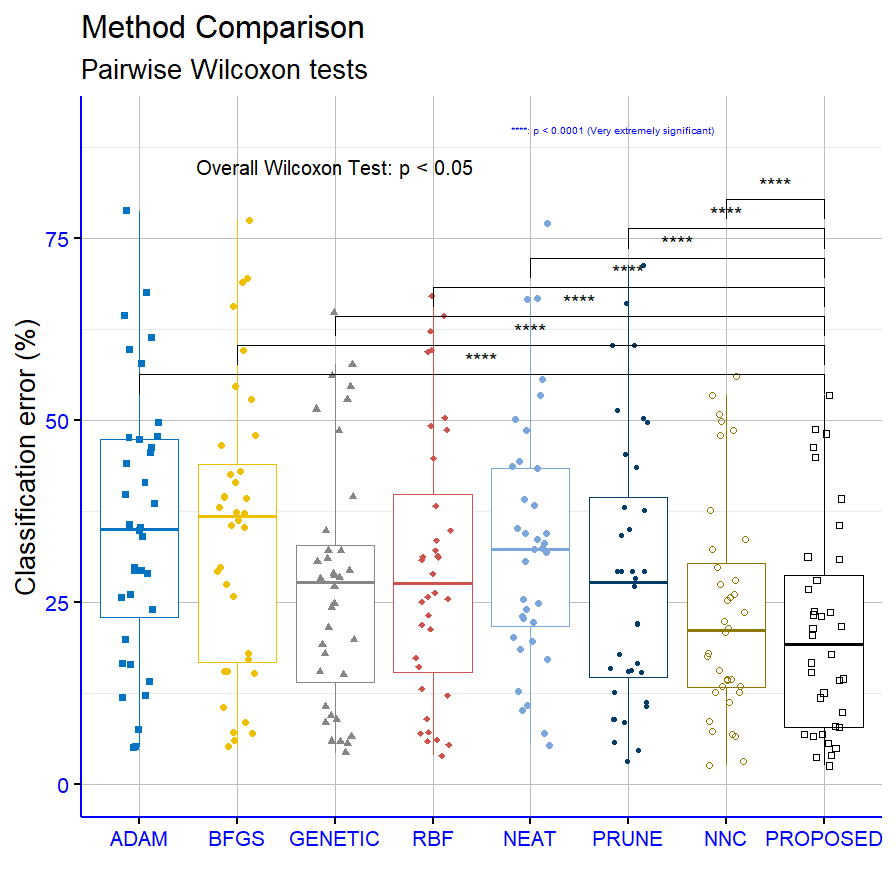
\includegraphics[scale=0.75]{new1}
\par\end{centering}
\caption{Statistical comparison of the machine learning models for the classification
datasets.\protect\label{fig:statClass}}

\end{figure}
In figure \ref{fig:statRegression}, all comparisons between the PROPOSED
model and other models show p-values significantly below the conventional
$0.05$ significance threshold, indicating statistically significant
differences. Specifically, the p-values are: PROPOSED vs ADAM = $0.00026$,
vs BFGS = $0.00084$, vs GENETIC = $0.0027$, vs RBF = $0.00068$,
vs NEAT = $1.9\times10^{-6}$, vs PRUNE = $0.00017$, and vs NNC =
$0.00011$. These values confirm that the PROPOSED model shows statistically
significant superiority over all compared models for regression datasets.
The particularly low p-value for NEAT ($1.9\times^{-6}$) highlights
a strong statistical difference, while the other comparisons also
maintain very small p-values, with only the GENETIC comparison showing
a slightly less pronounced (yet still statistically significant) difference
at p=0.0027. These results demonstrate that the PROPOSED model consistently
outperforms the others in regression tasks, with particularly marked
differences compared to models like NEAT, NNC and PRUNE. The consistency
of these findings reinforces the reliability of the PROPOSED model
and supports its use as the preferred method for similar regression
problems.

\begin{figure}[H]
\begin{centering}
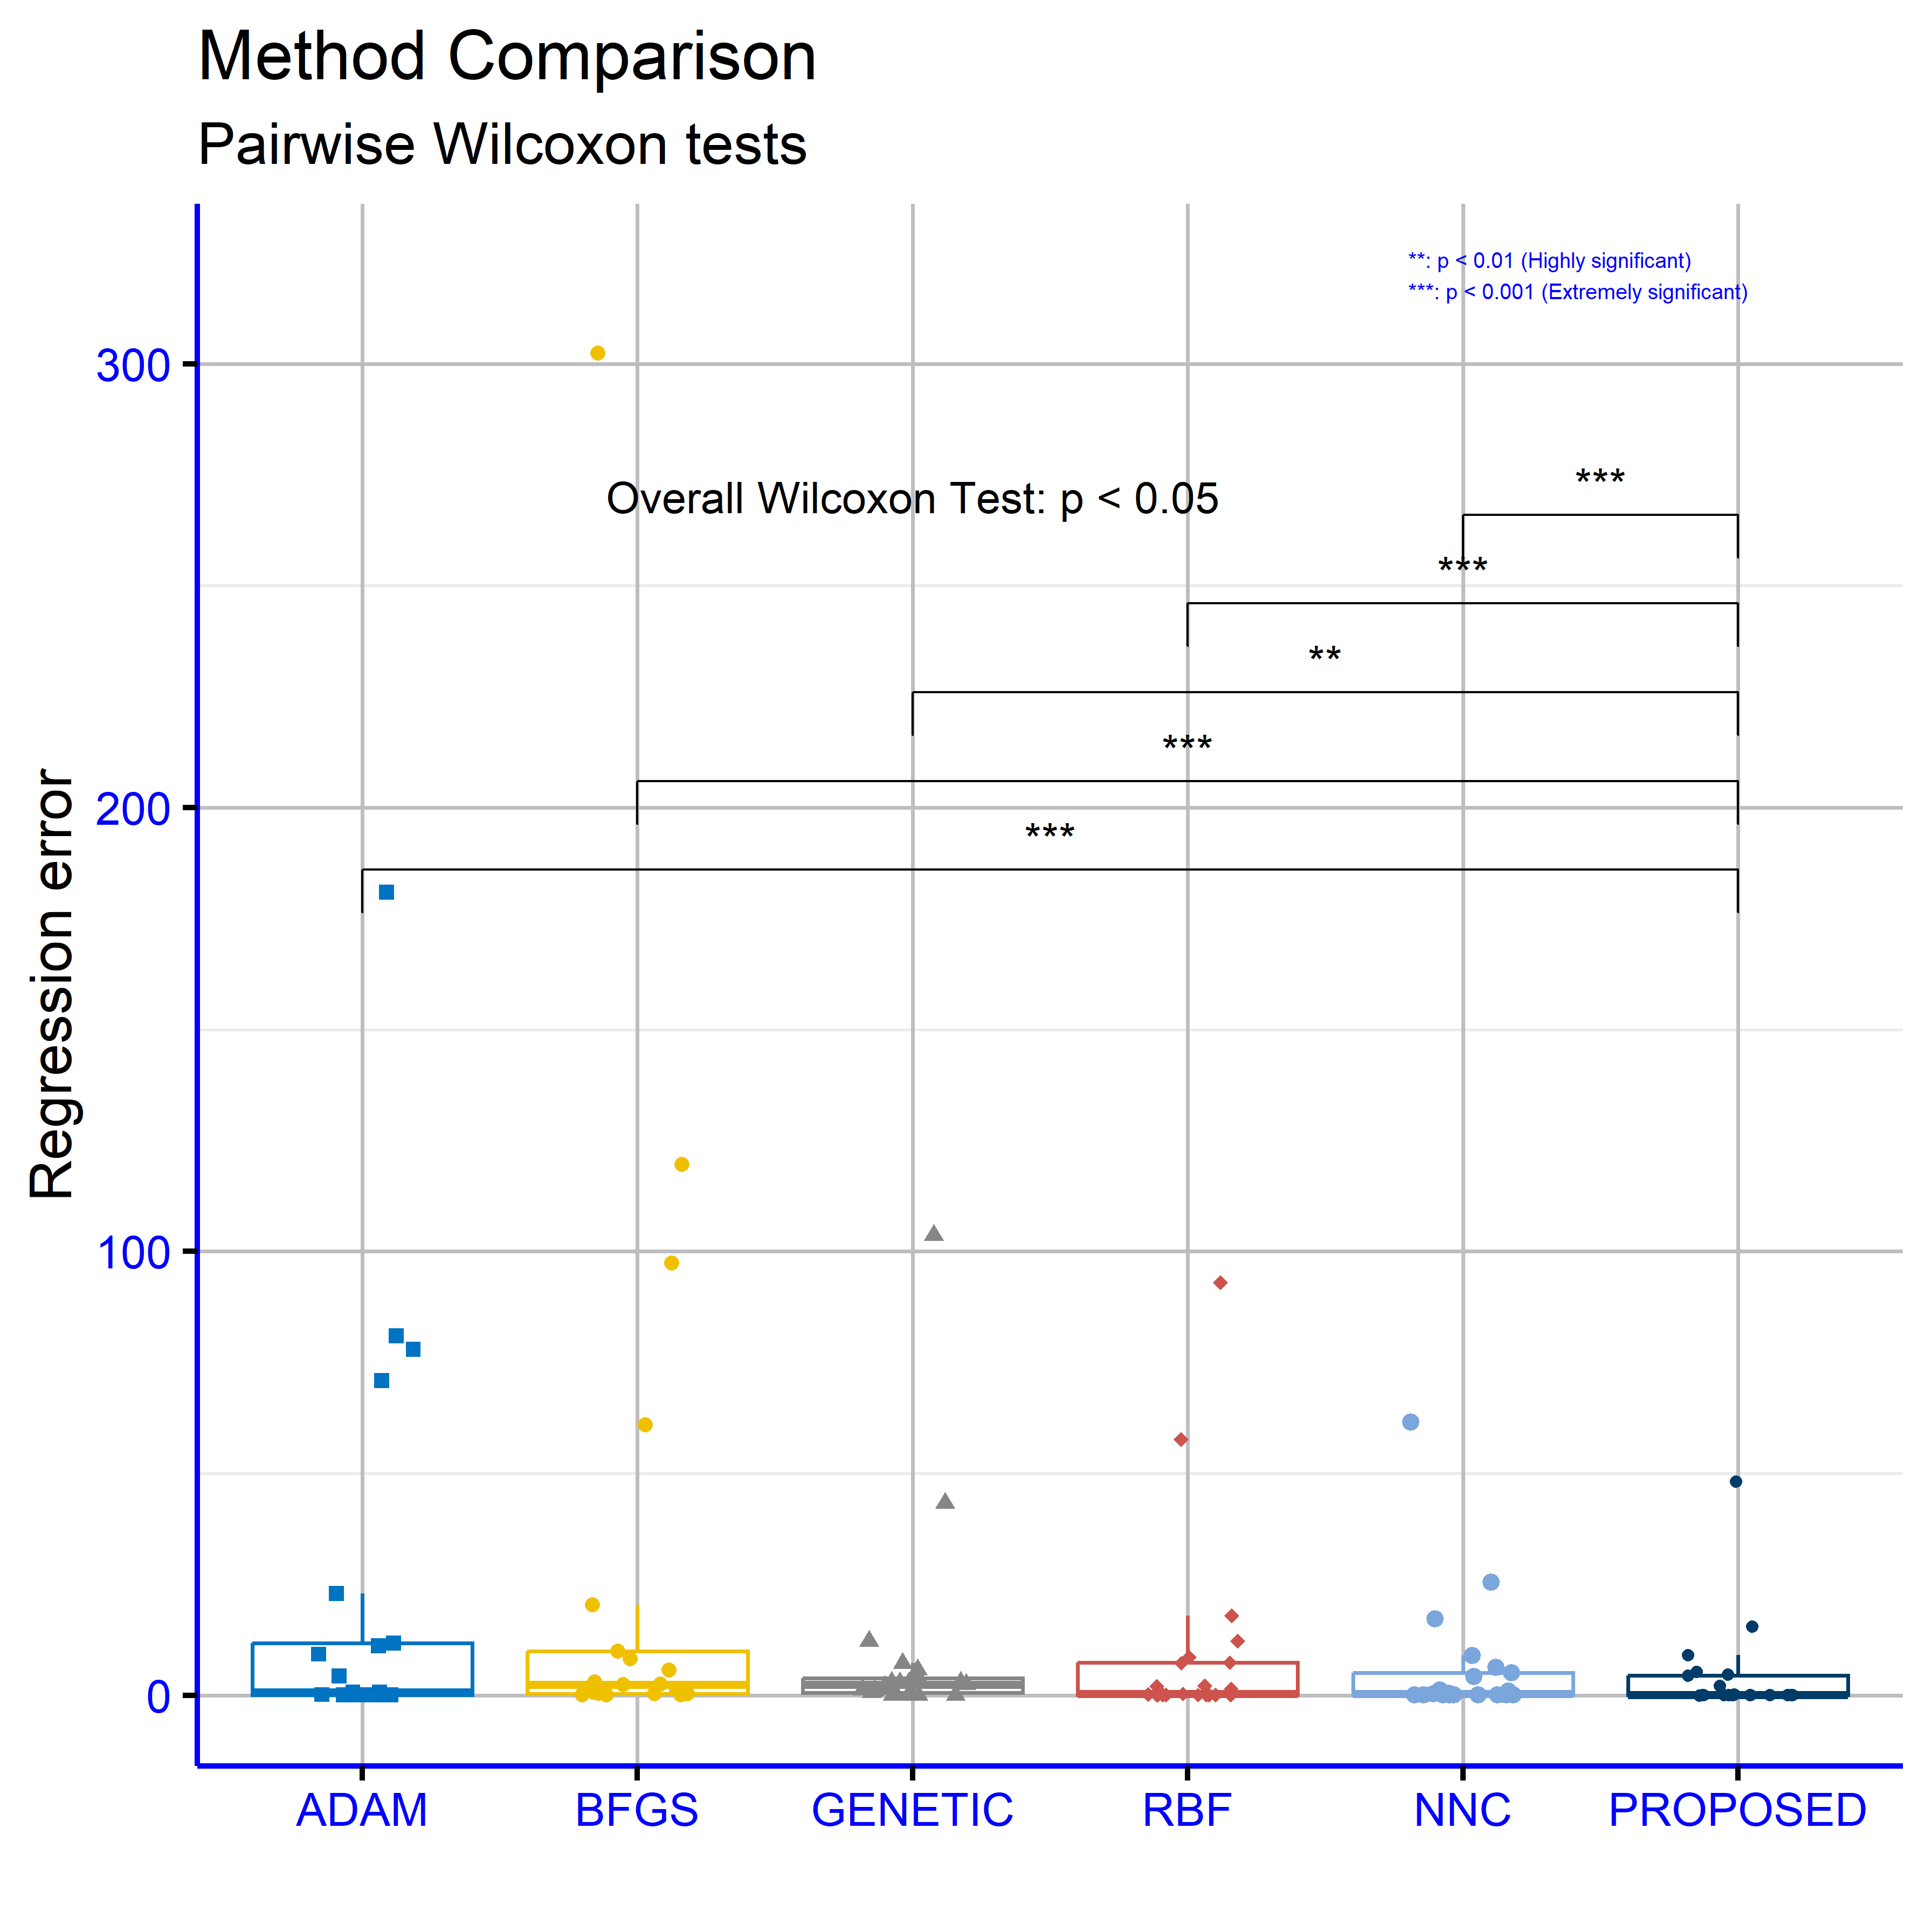
\includegraphics[scale=0.75]{new2}
\par\end{centering}
\caption{Statistical comparison between the used methods for the regression
datasets.\protect\label{fig:statRegression}}

\end{figure}
Also, in order to illustrated the robustness of the proposed method,
another experiment was conducted were the uniform crossover procedure
was used for the Neural Network Construction method and the proposed
one instead of the one - point crossover. The experimental results
for the classification datasets are shown in Table \ref{tab:experClassUniformOnePointVsCrossover}and
for regression datasets in Table \ref{tab:expersRegressionOnePointVsUniform}.

\begin{table}[H]
\caption{Experimental results for the classification datasets were a comparison
is made against the original one - point crossover method and the
uniform crossover procedure.\protect\label{tab:experClassUniformOnePointVsCrossover}}

\raggedright{}{\footnotesize{}%
\begin{tabular}{|c|c|c|c|c|}
\hline 
{\scriptsize DATASET} & {\scriptsize NNC ONE-POINT} & {\scriptsize NNC -UNIFORM} & {\scriptsize PROPOSED ONE-POINT} & {\scriptsize PROPOSED UNIFORM}\tabularnewline
\hline 
\hline 
{\footnotesize APPENDICITIS} & {\footnotesize 14.40\%} & {\footnotesize 14.20\%} & {\footnotesize 14.30\%} & {\footnotesize 14.40\%}\tabularnewline
\hline 
{\footnotesize ALCOHOL} & {\footnotesize 37.72\%} & {\footnotesize 42.34\%} & {\footnotesize 35.60\%} & {\footnotesize 39.70\%}\tabularnewline
\hline 
{\footnotesize AUSTRALIAN} & {\footnotesize 14.46\%} & {\footnotesize 14.13\%} & {\footnotesize 14.55\%} & {\footnotesize 14.35\%}\tabularnewline
\hline 
{\footnotesize BALANCE} & {\footnotesize 23.65\%} & {\footnotesize 20.73\%} & {\footnotesize 7.84\%} & {\footnotesize 7.61\%}\tabularnewline
\hline 
{\footnotesize CLEVELAND} & {\footnotesize 50.93\%} & {\footnotesize 51.45\%} & {\footnotesize 46.41\%} & {\footnotesize 46.28\%}\tabularnewline
\hline 
{\footnotesize CIRCULAR} & {\footnotesize 12.66\%} & {\footnotesize 17.59\%} & {\footnotesize 6.92\%} & {\footnotesize 11.86\%}\tabularnewline
\hline 
{\footnotesize DERMATOLOGY} & {\footnotesize 21.54\%} & {\footnotesize 30.09\%} & {\footnotesize 20.54\%} & {\footnotesize 26.86\%}\tabularnewline
\hline 
{\footnotesize ECOLI} & {\footnotesize 49.88\%} & {\footnotesize 48.12\%} & {\footnotesize 48.82\%} & {\footnotesize 48.88\%}\tabularnewline
\hline 
{\footnotesize GLASS} & {\footnotesize 56.09\%} & {\footnotesize 57.43\%} & {\footnotesize 53.52\%} & {\footnotesize 52.43\%}\tabularnewline
\hline 
{\footnotesize HABERMAN} & {\footnotesize 27.53\%} & {\footnotesize 27.17\%} & {\footnotesize 26.80\%} & {\footnotesize 26.70\%}\tabularnewline
\hline 
{\footnotesize HAYES-ROTH} & {\footnotesize 33.69\%} & {\footnotesize 36.61\%} & {\footnotesize 31.00\%} & {\footnotesize 33.62\%}\tabularnewline
\hline 
{\footnotesize HEART} & {\footnotesize 15.67\%} & {\footnotesize 16.41\%} & {\footnotesize 15.45\%} & {\footnotesize 14.96\%}\tabularnewline
\hline 
{\footnotesize HEARTATTACK} & {\footnotesize 20.87\%} & {\footnotesize 21.50\%} & {\footnotesize 21.77\%} & {\footnotesize 21.27\%}\tabularnewline
\hline 
{\footnotesize HOUSEVOTES} & {\footnotesize 3.17\%} & {\footnotesize 3.44\%} & {\footnotesize 3.78\%} & {\footnotesize 3.43\%}\tabularnewline
\hline 
{\footnotesize IONOSPHERE} & {\footnotesize 11.29\%} & {\footnotesize 11.80\%} & {\footnotesize 11.94\%} & {\footnotesize 11.77\%}\tabularnewline
\hline 
{\footnotesize LIVERDISORDER} & {\footnotesize 32.35\%} & {\footnotesize 32.65\%} & {\footnotesize 31.32\%} & {\footnotesize 32.32\%}\tabularnewline
\hline 
{\footnotesize LYMOGRAPHY} & {\footnotesize 25.29\%} & {\footnotesize 28.21\%} & {\footnotesize 23.72\%} & {\footnotesize 25.14\%}\tabularnewline
\hline 
{\footnotesize MAMMOGRAPHIC} & {\footnotesize 17.62\%} & {\footnotesize 18.04\%} & {\footnotesize 16.74\%} & {\footnotesize 16.24\%}\tabularnewline
\hline 
{\footnotesize PARKINSONS} & {\footnotesize 12.74\%} & {\footnotesize 11.63\%} & {\footnotesize 12.63\%} & {\footnotesize 12.74\%}\tabularnewline
\hline 
{\footnotesize PHONEME} & {\footnotesize 22.50\%} & {\footnotesize 23.46\%} & {\footnotesize 21.52\%} & {\footnotesize 21.32\%}\tabularnewline
\hline 
{\footnotesize PIMA} & {\footnotesize 28.07\%} & {\footnotesize 27.95\%} & {\footnotesize 23.34\%} & {\footnotesize 24.43\%}\tabularnewline
\hline 
{\footnotesize POPFAILURES} & {\footnotesize 6.98\%} & {\footnotesize 6.80\%} & {\footnotesize 5.72\%} & {\footnotesize 6.01\%}\tabularnewline
\hline 
{\footnotesize REGIONS2} & {\footnotesize 26.18\%} & {\footnotesize 25.71\%} & {\footnotesize 23.81\%} & {\footnotesize 25.21\%}\tabularnewline
\hline 
{\footnotesize SAHEART} & {\footnotesize 29.80\%} & {\footnotesize 30.52\%} & {\footnotesize 28.04\%} & {\footnotesize 29.13\%}\tabularnewline
\hline 
{\footnotesize SEGMENT} & {\footnotesize 53.50\%} & {\footnotesize 54.78\%} & {\footnotesize 48.20\%} & {\footnotesize 52.26\%}\tabularnewline
\hline 
{\footnotesize SPIRAL} & {\footnotesize 48.01\%} & {\footnotesize 48.35\%} & {\footnotesize 44.95\%} & {\footnotesize 45.03\%}\tabularnewline
\hline 
{\footnotesize STATHEART} & {\footnotesize 18.08\%} & {\footnotesize 18.85\%} & {\footnotesize 17.93\%} & {\footnotesize 18.59\%}\tabularnewline
\hline 
{\footnotesize STUDENT} & {\footnotesize 6.70\%} & {\footnotesize 6.15\%} & {\footnotesize 4.05\%} & {\footnotesize 4.10\%}\tabularnewline
\hline 
{\footnotesize TRANSFUSION} & {\footnotesize 25.77\%} & {\footnotesize 25.58\%} & {\footnotesize 23.16\%} & {\footnotesize 23.96\%}\tabularnewline
\hline 
{\footnotesize WDBC} & {\footnotesize 7.36\%} & {\footnotesize 8.07\%} & {\footnotesize 4.95\%} & {\footnotesize 6.31\%}\tabularnewline
\hline 
{\footnotesize WINE} & {\footnotesize 13.59\%} & {\footnotesize 14.41\%} & {\footnotesize 9.94\%} & {\footnotesize 11.76\%}\tabularnewline
\hline 
{\footnotesize Z\_F\_S} & {\footnotesize 14.53\%} & {\footnotesize 18.33\%} & {\footnotesize 7.97\%} & {\footnotesize 10.13\%}\tabularnewline
\hline 
{\footnotesize Z\_O\_N\_F\_S} & {\footnotesize 48.62\%} & {\footnotesize 51.10\%} & {\footnotesize 39.28\%} & {\footnotesize 44.90\%}\tabularnewline
\hline 
{\footnotesize ZO\_NF\_S} & {\footnotesize 13.54\%} & {\footnotesize 14.52\%} & {\footnotesize 6.94\%} & {\footnotesize 8.24\%}\tabularnewline
\hline 
{\footnotesize ZONF\_S} & {\footnotesize 2.64\%} & {\footnotesize 2.82\%} & {\footnotesize 2.60\%} & {\footnotesize 2.78\%}\tabularnewline
\hline 
{\footnotesize ZOO} & {\footnotesize 8.70\%} & {\footnotesize 10.40\%} & {\footnotesize 6.60\%} & {\footnotesize 8.70\%}\tabularnewline
\hline 
{\footnotesize\textbf{AVERAGE}} & {\footnotesize\textbf{24.79\%}} & {\footnotesize\textbf{24.76\%}} & {\footnotesize\textbf{21.18\%}} & {\footnotesize\textbf{22.32\%}}\tabularnewline
\hline 
\end{tabular}}{\footnotesize\par}
\end{table}
\begin{table}[H]

\caption{Experimental results for the regression datasets using two crossover
methods: the one point crossover and the uniform crossover. \protect\label{tab:expersRegressionOnePointVsUniform}}

\centering{}{\footnotesize{}%
\begin{tabular}{|c|c|c|c|c|}
\hline 
{\footnotesize DATASET} & {\footnotesize NNC ONE-POINT} & {\footnotesize NNC UNIFORM} & {\footnotesize PROPOSED ONE-POINT} & {\footnotesize PROPOSED UNIFORM}\tabularnewline
\hline 
\hline 
{\footnotesize ABALONE} & {\footnotesize 5.08} & {\footnotesize 5.40} & {\footnotesize 4.47} & {\footnotesize 4.55}\tabularnewline
\hline 
{\footnotesize AIRFOIL} & {\footnotesize 0.004} & {\footnotesize 0.004} & {\footnotesize 0.002} & {\footnotesize 0.003}\tabularnewline
\hline 
{\footnotesize AUTO} & {\footnotesize 17.13} & {\footnotesize 20.06} & {\footnotesize 9.09} & {\footnotesize 11.10}\tabularnewline
\hline 
{\footnotesize BK} & {\footnotesize 0.10} & {\footnotesize 0.018} & {\footnotesize 0.023} & {\footnotesize 0.018}\tabularnewline
\hline 
{\footnotesize BL} & {\footnotesize 1.19} & {\footnotesize 0.018} & {\footnotesize 0.001} & {\footnotesize 0.001}\tabularnewline
\hline 
{\footnotesize BASEBALL} & {\footnotesize 61.57} & {\footnotesize 63.44} & {\footnotesize 48.13} & {\footnotesize 49.99}\tabularnewline
\hline 
{\footnotesize CONCRETE} & {\footnotesize 0.008} & {\footnotesize 0.009} & {\footnotesize 0.005} & {\footnotesize 0.006}\tabularnewline
\hline 
{\footnotesize DEE} & {\footnotesize 0.26} & {\footnotesize 0.28} & {\footnotesize 0.22} & {\footnotesize 0.24}\tabularnewline
\hline 
{\footnotesize FRIEDMAN} & {\footnotesize 6.29} & {\footnotesize 6.98} & {\footnotesize 5.34} & {\footnotesize 5.85}\tabularnewline
\hline 
{\footnotesize FY} & {\footnotesize 0.11} & {\footnotesize 0.04} & {\footnotesize 0.043} & {\footnotesize 0.04}\tabularnewline
\hline 
{\footnotesize HO} & {\footnotesize 0.015} & {\footnotesize 0.016} & {\footnotesize 0.016} & {\footnotesize 0.011}\tabularnewline
\hline 
{\footnotesize HOUSING} & {\footnotesize 25.47} & {\footnotesize 26.68} & {\footnotesize 15.47} & {\footnotesize 16.89}\tabularnewline
\hline 
{\footnotesize LASER} & {\footnotesize 0.025} & {\footnotesize 0.041} & {\footnotesize 0.0049} & {\footnotesize 0.008}\tabularnewline
\hline 
{\footnotesize LW} & {\footnotesize 0.011} & {\footnotesize 0.012} & {\footnotesize 0.011} & {\footnotesize 0.011}\tabularnewline
\hline 
{\footnotesize MORTGAGE} & {\footnotesize 0.30} & {\footnotesize 0.29} & {\footnotesize 0.023} & {\footnotesize 0.037}\tabularnewline
\hline 
{\footnotesize PL} & {\footnotesize 0.047} & {\footnotesize 0.046} & {\footnotesize 0.029} & {\footnotesize 0.024}\tabularnewline
\hline 
{\footnotesize PLASTIC} & {\footnotesize 4.20} & {\footnotesize 5.20} & {\footnotesize 2.17} & {\footnotesize 2.30}\tabularnewline
\hline 
{\footnotesize QUAKE} & {\footnotesize 0.96} & {\footnotesize 0.036} & {\footnotesize 0.036} & {\footnotesize 0.036}\tabularnewline
\hline 
{\footnotesize SN} & {\footnotesize 0.026} & {\footnotesize 0.026} & {\footnotesize 0.024} & {\footnotesize 0.024}\tabularnewline
\hline 
{\footnotesize STOCK} & {\footnotesize 8.92} & {\footnotesize 10.89} & {\footnotesize 4.69} & {\footnotesize 8.31}\tabularnewline
\hline 
{\footnotesize TREASURY} & {\footnotesize 0.43} & {\footnotesize 0.38} & {\footnotesize 0.068} & {\footnotesize 0.072}\tabularnewline
\hline 
{\footnotesize\textbf{AVERAGE}} & {\footnotesize\textbf{6.29}} & {\footnotesize\textbf{6.66}} & {\footnotesize\textbf{4.28}} & {\footnotesize\textbf{4.74}}\tabularnewline
\hline 
\end{tabular}}{\footnotesize\par}
\end{table}
Analysis of the results in Table \ref{tab:experClassUniformOnePointVsCrossover}
demonstrates that the proposed method systematically outperforms both
variants of NNC, regardless of the crossover type employed. Specifically,
the proposed method with one-point crossover achieves a significantly
lower average error rate (21.18\%) compared to NNC (24.79\%). A similar
performance gap is observed with uniform crossover, where the proposed
method maintains superiority (22.32\% vs NNC's 24.76\%). The advantage
is particularly pronounced in several datasets: for BALANCE (7.61-7.84\%
vs 20.73-23.65\%), CIRCULAR (6.92-11.86\% vs 12.66-17.59\%), Z\_F\_S
(7.97-10.13\% vs 14.53-18.33\%), and ZO\_NF\_S (6.94-8.24\% vs 13.54-14.52\%).
Notably, in datasets like WDBC and WINE, the proposed method reduces
the error by nearly half compared to NNC. Interestingly, the choice
of crossover type shows minimal impact on performance for both methods.
The marginal differences between one-point and uniform crossover (with
average errors remaining stable for each method) suggest that the
proposed method's superiority stems from its fundamental architecture
rather than the recombination technique. These experimental results
confirm the robustness of the proposed method, which maintains consistent
superiority across various classification datasets while significantly
reducing average error rates compared to standard NNC approaches.

Table \ref{tab:expersRegressionOnePointVsUniform} further validates
the proposed method's superiority for regression datasets. The proposed
method achieves lower average errors with both one-point (4.28) and
uniform crossover (4.74) compared to NNC (6.29 and 6.66 respectively).
The performance gap is especially notable in key datasets: AUTO (9.09-11.1
vs 17.13-20.06), HOUSING (15.47-16.89 vs 25.47-26.68), and PLASTIC
(2.17-2.3 vs 4.2-5.2). In several cases (AIRFOIL, LASER, MORTGAGE),
the proposed method reduces errors to a fraction of NNC's values.
Particularly impressive results appear in BL (0.001) and QUAKE (0.036),
where the proposed method achieves remarkably low, crossover-invariant
errors. The crossover type shows slightly less impact on the proposed
method (average difference of 0.46) than on NNC (0.37 difference),
though one-point crossover yields marginally better results for both.
These comprehensive results confirm that the proposed method maintains
its superiority in regression problems, delivering consistently and
significantly improved performance over NNC. Its ability to achieve
lower errors across diverse problems, independent of crossover selection,
solidifies its position as a more reliable and effective approach.

Another experiment was conducted where the parameter $N_{K}$ was
altered in the range $[5,\ldots,50]$ and the results for the regression
datasets are depicted in Figure \ref{fig:nkExpers}.

\begin{figure}[H]
\begin{centering}
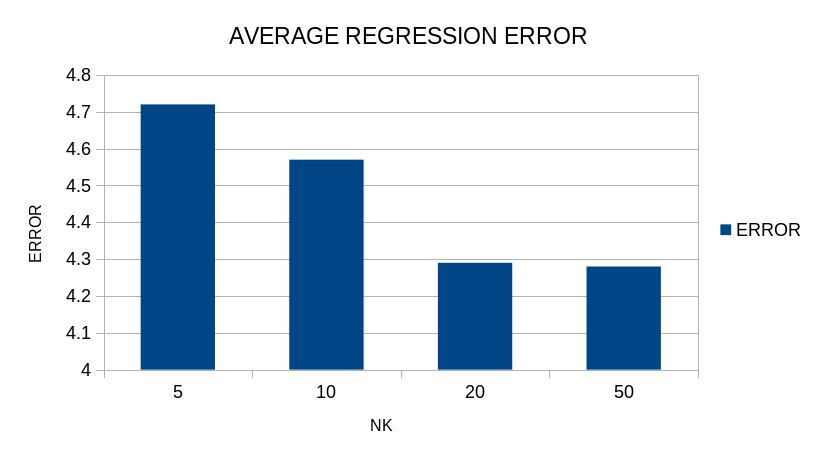
\includegraphics[scale=0.5]{nk_exper}
\par\end{centering}
\caption{Average regression error for the regression datasets and the proposed
method using a variety of values for the parameter $N_{K}$.\protect\label{fig:nkExpers}}

\end{figure}
Additionally a series of experiments was conducted where the parameter
$N_{I}$ was changed from 10 to 40 and the results are graphically
presented in Figure \ref{fig:expersNI}.
\begin{figure}[H]
\begin{centering}
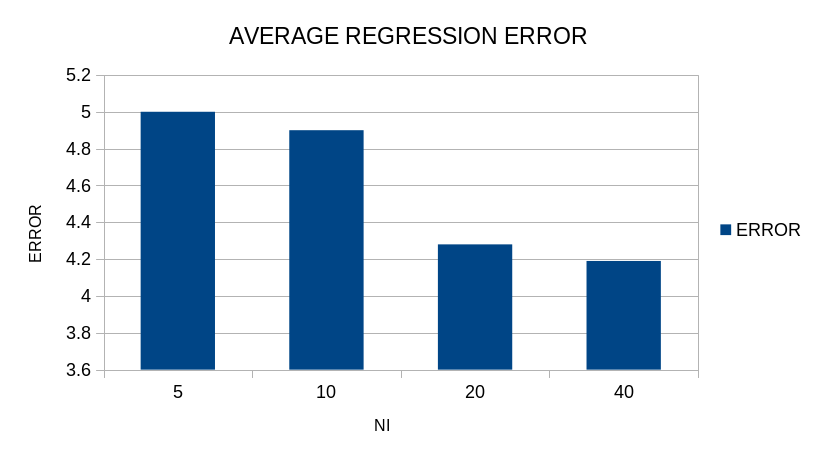
\includegraphics[scale=0.5]{ni_exper}
\par\end{centering}
\caption{Experimental results for the regression datasets and the proposed
method using a variety of values for the parameter $N_{I}$.\protect\label{fig:expersNI}}

\end{figure}
 This figure presents the relationship between the number of chromosomes
($N_{I}$) participating in the secondary genetic algorithm and the
resulting regression error. We observe that as the number of chromosomes
increases, the error decreases, indicating improvement in the model's
performance. Specifically, for $N_{I}=5$, the error is 4.99, while
for $N_{I}=10$, the error drops to 4.89. This trend continues with
further increase in chromosomes: for $N_{I}=20$, the error reaches
4.27, and for $N_{I}=40$, the error reaches 4.18. This error reduction
shows that using more chromosomes in the secondary genetic algorithm
leads to better optimization of the neural network's parameters, resulting
in error minimization. However, the improvement is not linear. We
observe that the difference in error between $N_{I}=5$ and $N_{I}=10$
is 0.10, while between $N_{I}=20$ and $N_{I}=40$ it is only 0.09.
This may indicate that beyond a certain point, increasing chromosomes
has progressively smaller impact on error reduction. This phenomenon
may be due to factors such as algorithm convergence or the existence
of an optimization threshold beyond which improvement becomes more
difficult. Furthermore, the selection of $N_{I}$ may be influenced
by computational constraints. Using more chromosomes increases the
computational load, so the performance improvement must be balanced
against resource costs. For example, transitioning from $N_{I}=20$
to $N_{I}=40$ leads to error reduction of only 0.09, which may not
justify the doubling of computational cost in certain scenarios. In
summary, the table confirms that increasing the number of chromosomes
improves the model's performance, but its effect becomes smaller as
$N_{I}$ grows larger. This means that the optimal selection of $N_{I}$
depends on a combination of factors, such as the desired accuracy,
available computational resources, and the nature of the problem. 

Furthermore, as a practical example of application, consider the prediction
of the duration of forest fires as presented for the Greek territory
in a recent publication \citep{ml_fire}. Using data from the Greek
Fire Service, an attempt is made to predict the duration of forest
fires for the years 2014-2023. Figure \ref{fig:mlFire} depicts a
comparison for the classification error for this problem for the years
2014-2023 between the original Neural Network Construction method,
denoted as NNC and the proposed method which is denoted as NNC\_GA
in the plot. 
\begin{figure}[H]
\begin{centering}
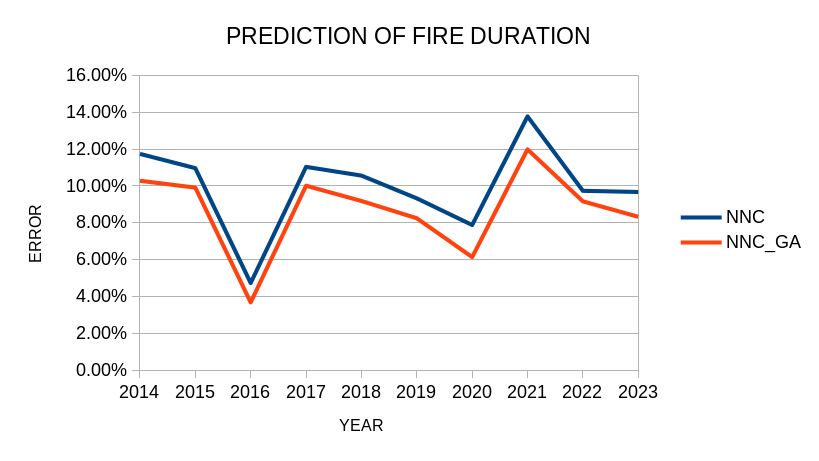
\includegraphics[scale=0.5]{ml_fire}
\par\end{centering}
\caption{Comparison of the original NNC method and the proposed modification
(NNC\_GA) for the prediction of forest fires for the Greek teritory.
The horizontal axis denotes the year and the vertical the obtained
classification error.\protect\label{fig:mlFire}}

\end{figure}
 As is evident, the proposed method has a lower error in estimating
the duration of forest fires in all years from 2014 to 2023 compared
to the original artificial neural network construction technique.

\section{Discussion \protect\label{sec:Discussion}}

This study presents an interesting approach combining grammatical
evolution with modified genetic algorithms for constructing artificial
neural networks. However, a comprehensive analysis of the results
and practical implications reveals several aspects that require further
investigation and critical examination. While the experimental findings
demonstrate certain improvements over traditional techniques, the
interpretation and significance of these improvements have not been
analyzed with the depth and critical thinking required for a complete
method evaluation. Regarding classification performance, the method
shows an average error rate of 21.18\% compared to ADAM's 36.45\%
and BFGS's 35.71\%. However, these comparative metrics conceal significant
performance variations across different datasets. For instance, on
Cleveland and Ecoli datasets, classification error reaches 46.41\%
and 48.82\% respectively, while on Housevotes and Zoo it drops below
7\%. This substantial performance variation suggests the method may
be highly sensitive to dataset-specific characteristics, which isn't
sufficiently analyzed in the results presentation. Furthermore, the
lack of analysis regarding variation across the 30 repetitions of
each experiment raises questions about the method's stability and
reliability in real-world applications.The statistical significance
of results, while supported by extremely low p-values (1.9e-07 to
1.1e-08), doesn't account for the dynamics of different problem types.
In noisy datasets or those with significant class imbalance like Haberman
and Liverdisorder, the method shows notable performance fluctuations
that remain unexplained. Additionally, the absence of analysis regarding
dataset characteristics affecting performance (such as dimensionality,
sample size, or degree of linear separability) makes it difficult
to determine the optimal conditions for the method's application.Computational
resources and execution times present another critical but underexplored
issue. 

While the study mentions using an AMD Ryzen 5950X system with 128GB
RAM, comprehensive reporting of computational requirements is missing.
Specifically, it would be essential to present average training times
per dataset category (classification vs regression), the method's
scalability regarding number of features and samples, memory consumption
during the grammatical evolution process, and the impact of various
parameters (like population size and generation count) on execution
times. This lack of information makes practical implementation assessment
challenging, especially for real-world problems where computational
resources and time constraints are crucial factors. Regarding limitations,
while the study acknowledges issues like local optima and overfitting,
their analysis remains superficial. For example, in datasets like
Z\_O\_N\_F\_S with 39.28\% error, it's not investigated whether this
results from insufficient solution space exploration due to grammatical
evolution parameters, limitations in the grammar used for architecture
generation, excessive network complexity leading to overfitting, or
inadequacies in parameter training mechanisms.Practical application
and robustness require more thorough examination. Beyond controlled
experimental scenarios, there's missing information about the ease
of applying the method to real-world, unprocessed datasets, the required
expertise for optimal parameter tuning, the method's resilience to
noisy, incomplete or imbalanced data, and the interpretability of
results and generated architectures.Moreover, comparisons with contemporary
approaches like transformers, convolutional neural networks, or reinforcement
learning methods in domains where they dominate (e.g., natural language
processing, computer vision, robotics) are completely absent from
the study. This evaluation gap significantly limits our understanding
of the method's relative value compared to state-of-the-art alternatives.
The method's generalizability to new application domains hasn't been
adequately explored. While results are presented across various fields
(medicine, physics, economics), critical information is missing about
the flexibility and adaptability of the used grammar across different
domains, required modifications for new data types (time series, graphs,
spatial data), knowledge transfer capability between different applications,
and domain knowledge requirements for appropriate grammar design.
In summary, while the proposed method introduces interesting mechanisms
for improving automated neural network design, this analysis reveals
numerous aspects needing further investigation. 

For a complete and objective evaluation, it would be necessary to
conduct a much more detailed analysis of result stability and variation,
comparisons with alternative contemporary approaches beyond the basic
techniques examined, thorough evaluation of scalability and computational
requirements for large datasets, in-depth investigation of real-world
implementation challenges and limitations, and analysis of generalization
and adaptation capability to new domains and data types. Only through
such a holistic and critical approach could we obtain a complete picture
of this methodology's value, capabilities and limitations. The current
results, while encouraging, leave significant gaps in our understanding
of how and under what conditions the method can truly provide value
compared to existing approaches in automated neural network design.

\section{Conclusions\protect\label{sec:Conclusions}}

The article presents a method for constructing artificial neural networks
by integrating Grammatical Evolution (GE) with a modified Genetic
Algorithm (GA) to improve generalization properties and reduce overfitting.
The method proves to be effective in designing neural network architectures
and optimizing their parameters. The modified genetic algorithm avoids
local minima during training and addresses overfitting by applying
penalty factors to the fitness function, ensuring better generalization
to unseen data. The method was evaluated on a variety of classification
and regression datasets from diverse fields, including physics, chemistry,
medicine, and economics. Comparative results indicate that the proposed
method achieves lower error rates on average compared to traditional
optimization and machine learning techniques, highlighting its stability
and adaptability. The results, analyzed through statistical metrics
such as p-values, provide strong evidence of the method’s superiority
over competing models in both classification and regression tasks.
A key innovation of the method is the combination of dynamic architecture
generation and parameter optimization within a unified framework.
This approach not only enhances performance but also reduces the computational
complexity associated with manually designing neural networks. Additionally,
the use of constraint techniques in the genetic algorithm ensures
the preservation of the neural network structure while enabling controlled
optimization of parameters. Future explorations could focus on testing
the method on larger and more complex datasets, such as those encountered
in image recognition, natural language processing, and genomics, to
evaluate its scalability and effectiveness in real-world applications.
Furthermore, the integration of other global optimization methods,
such as Particle Swarm Optimization, Simulated Annealing, or Differential
Evolution, could be considered to further enhance the algorithm’s
robustness and convergence speed. Concurrently, the inclusion of regularization
techniques, such as dropout or batch normalization, could improve
the method’s generalization capabilities even further. Reducing computational
cost is another important area of investigation, and the method could
be adapted to leverage parallel computing architectures, such as GPUs
or distributed systems, making it feasible for training on large datasets
or for real-time applications. Finally, customizing the grammar used
in Grammatical Evolution based on the specific characteristics of
individual fields could improve the method’s performance in specialized
tasks, such as time-series forecasting or anomaly detection in cybersecurity.

\vspace{6pt}


\authorcontributions{V.C. and I.G.T. conducted the experiments, employing several datasets
and provided the comparative experiments. D.T. and V.C. performed
the statistical analysis and prepared the manuscript. All authors
have read and agreed to the published version of the manuscript.}

\funding{This research received no external funding.}

\institutionalreview{Not applicable.}

\institutionalreview{Not applicable.}

\institutionalreview{Not applicable.}

\acknowledgments{This research has been financed by the European Union : Next Generation
EU through the Program Greece 2.0 National Recovery and Resilience
Plan , under the call RESEARCH -- CREATE -- INNOVATE, project name
“iCREW: Intelligent small craft simulator for advanced crew training
using Virtual Reality techniques\textquotedbl{} (project code:TAEDK-06195).}

\conflictsofinterest{The authors declare no conflicts of interest.}

\begin{adjustwidth}{-\extralength}{0cm}{}

\reftitle{References}
\begin{thebibliography}{99}
\bibitem{nn1}Abiodun, O. I., Jantan, A., Omolara, A. E., Dada, K.
V., Mohamed, N. A., \& Arshad, H. (2018). State-of-the-art in artificial
neural network applications: A survey. Heliyon, 4(11).

\bibitem{nn2}Suryadevara, S., \& Yanamala, A. K. Y. (2021). A Comprehensive
Overview of Artificial Neural Networks: Evolution, Architectures,
and Applications. Revista de Inteligencia Artificial en Medicina,
12(1), 51-76.

\bibitem{nn_image}M. Egmont-Petersen, D. de Ridder, H. Handels, Image
processing with neural networks---a review, Pattern Recognition \textbf{35},
pp. 2279-2301, 2002.

\bibitem{nn_timeseries}G.Peter Zhang, Time series forecasting using
a hybrid ARIMA and neural network model, Neurocomputing \textbf{50},
pp. 159-175, 2003.

\bibitem{nn_credit}Z. Huang, H. Chen, C.-Jung Hsu, W.-Hwa Chen, S.
Wu, Credit rating analysis with support vector machines and neural
networks: a market comparative study, Decision Support Systems \textbf{37},
pp. 543-558, 2004.

\bibitem{nnphysics1}P. Baldi, K. Cranmer, T. Faucett et al, Parameterized
neural networks for high-energy physics, Eur. Phys. J. C \textbf{76},
2016.

\bibitem{nnphysics2}Baldi, P., Cranmer, K., Faucett, T., Sadowski,
P., \& Whiteson, D. (2016). Parameterized neural networks for high-energy
physics. The European Physical Journal C, 76(5), 1-7.

\bibitem{bpnn1}Vora, K., \& Yagnik, S. (2014). A survey on backpropagation
algorithms for feedforward neural networks. International Journal
of Engineering Development and Research, 1(3), 193-197.

\bibitem{bpnn2}K. Vora, S. Yagnik, A survey on backpropagation algorithms
for feedforward neural networks, International Journal of Engineering
Development and Research \textbf{1}, pp. 193-197, 2014.

\bibitem{rpropnn-1}Pajchrowski, T., Zawirski, K., \& Nowopolski,
K. (2014). Neural speed controller trained online by means of modified
RPROP algorithm. IEEE transactions on industrial informatics, 11(2),
560-568.

\bibitem{rpropnn-2}Hermanto, R. P. S., \& Nugroho, A. (2018). Waiting-time
estimation in bank customer queues using RPROP neural networks. Procedia
Computer Science, 135, 35-42.

\bibitem{nn_adam}D. P. Kingma, J. L. Ba, ADAM: a method for stochastic
optimization, in: Proceedings of the 3rd International Conference
on Learning Representations (ICLR 2015), pp. 1--15, 2015.

\bibitem{geneticnn1}Reynolds, J., Rezgui, Y., Kwan, A., \& Piriou,
S. (2018). A zone-level, building energy optimisation combining an
artificial neural network, a genetic algorithm, and model predictive
control. Energy, 151, 729-739.

\bibitem{psonn}Das, G., Pattnaik, P. K., \& Padhy, S. K. (2014).
Artificial neural network trained by particle swarm optimization for
non-linear channel equalization. Expert Systems with Applications,
41(7), 3491-3496.

\bibitem{nn_siman}Sexton, R. S., Dorsey, R. E., \& Johnson, J. D.
(1999). Beyond backpropagation: using simulated annealing for training
neural networks. Journal of Organizational and End User Computing
(JOEUC), 11(3), 3-10.

\bibitem{weight_de1}Wang, L., Zeng, Y., \& Chen, T. (2015). Back
propagation neural network with adaptive differential evolution algorithm
for time series forecasting. Expert Systems with Applications, 42(2),
855-863.

\bibitem{nn_abc}Karaboga, D., \& Akay, B. (2007, June). Artificial
bee colony (ABC) algorithm on training artificial neural networks.
In 2007 IEEE 15th Signal Processing and Communications Applications
(pp. 1-4). IEEE.

\bibitem{tabunn}R.S. Sexton, B. Alidaee, R.E. Dorsey, J.D. Johnson,
Global optimization for artificial neural networks: A tabu search
application. European Journal of Operational Research \textbf{106},
pp. 570-584, 1998.

\bibitem{nn_hybrid}J.-R. Zhang, J. Zhang, T.-M. Lok, M.R. Lyu, A
hybrid particle swarm optimization--back-propagation algorithm for
feedforward neural network training, Applied Mathematics and Computation
\textbf{185}, pp. 1026-1037, 2007.

\bibitem{nn_cascade}G. Zhao, T. Wang, Y. Jin, C. Lang, Y. Li, H.
Ling, The Cascaded Forward algorithm for neural network training,
Pattern Recognition \textbf{161}, 111292, 2025.

\bibitem{nn_gpu1}K-Su Oh, K. Jung, GPU implementation of neural networks,
Pattern Recognition \textbf{37}, pp. 1311-1314, 2004.

\bibitem{nn_gpu2}M. Zhang, K. Hibi, J. Inoue, GPU-accelerated artificial
neural network potential for molecular dynamics simulation, Computer
Physics Communications \textbf{285}, 108655, 2023. 

\bibitem{nnsharing1}S.J. Nowlan and G.E. Hinton, Simplifying neural
networks by soft weight sharing, Neural Computation 4, pp. 473-493,
1992.

\bibitem{nnsharing2}Nowlan, S. J., \& Hinton, G. E. (2018). Simplifying
neural networks by soft weight sharing. In The mathematics of generalization
(pp. 373-394). CRC Press.

\bibitem{nnprunning1}S.J. Hanson and L.Y. Pratt, Comparing biases
for minimal network construction with back propagation, In D.S. Touretzky
(Ed.), Advances in Neural Information Processing Systems, Volume 1,
pp. 177-185, San Mateo, CA: Morgan Kaufmann, 1989.

\bibitem{nnprunning2}M. Augasta and T. Kathirvalavakumar, Pruning
algorithms of neural networks --- a comparative study, Central European
Journal of Computer Science, 2003.

\bibitem{nnearly1}Lutz Prechelt, Automatic early stopping using cross
validation: quantifying the criteria, Neural Networks \textbf{11},
pp. 761-767, 1998.

\bibitem{nnearly2}X. Wu and J. Liu, A New Early Stopping Algorithm
for Improving Neural Network Generalization, 2009 Second International
Conference on Intelligent Computation Technology and Automation, Changsha,
Hunan, 2009, pp. 15-18.

\bibitem{nndecay1}N. K. Treadgold and T. D. Gedeon, Simulated annealing
and weight decay in adaptive learning: the SARPROP algorithm,IEEE
Transactions on Neural Networks \textbf{9}, pp. 662-668, 1998.

\bibitem{nndecay2}M. Carvalho and T. B. Ludermir, Particle Swarm
Optimization of Feed-Forward Neural Networks with Weight Decay, 2006
Sixth International Conference on Hybrid Intelligent Systems (HIS'06),
Rio de Janeiro, Brazil, 2006, pp. 5-5.

\bibitem{nn_arch1}J. Arifovic, R. Gençay, Using genetic algorithms
to select architecture of a feedforward artificial neural network,
Physica A: Statistical Mechanics and its Applications \textbf{289},
pp. 574-594, 2001.

\bibitem{nn_arch2}P.G. Benardos, G.C. Vosniakos, Optimizing feedforward
artificial neural network architecture, Engineering Applications of
Artificial Intelligence \textbf{20}, pp. 365-382, 2007.

\bibitem{nn_arch3}B.A. Garro, R.A. Vázquez, Designing Artificial
Neural Networks Using Particle Swarm Optimization Algorithms, Computational
Intelligence and Neuroscience, 369298, 2015. 

\bibitem[(2001)]{nn_ereinf}Siebel, N. T., \& Sommer, G. (2007). Evolutionary
reinforcement learning of artificial neural networks. International
Journal of Hybrid Intelligent Systems, 4(3), 171-183.

\bibitem[(2001)]{nn_reinf}Jaafra, Y., Laurent, J. L., Deruyver, A.,
\& Naceur, M. S. (2019). Reinforcement learning for neural architecture
search: A review. Image and Vision Computing, 89, 57-66.

\bibitem[(2001)]{nn_param_sharing}Pham, H., Guan, M., Zoph, B., Le,
Q., \& Dean, J. (2018, July). Efficient neural architecture search
via parameters sharing. In International conference on machine learning
(pp. 4095-4104). PMLR.

\bibitem[(2001)]{nn_snas}Xie, S., Zheng, H., Liu, C., \& Lin, L.
(2018). SNAS: stochastic neural architecture search. arXiv preprint
arXiv:1812.09926.

\bibitem[(2001)]{nn_bayes}Zhou, H., Yang, M., Wang, J., \& Pan, W.
(2019, May). Bayesnas: A bayesian approach for neural architecture
search. In International conference on machine learning (pp. 7603-7613).
PMLR.

\bibitem[(2001)]{nn_drug}L. Terfloth, J. Gasteige, Neural networks
and genetic algorithms in drug design, Drug Discovery Today \textbf{6},
pp. 102-108, 2001.

\bibitem[(2001)]{nn_estimates}Kim, G. H., Seo, D. S., \& Kang, K.
I. (2005). Hybrid models of neural networks and genetic algorithms
for predicting preliminary cost estimates. Journal of computing in
civil engineering, 19(2), 208-211.

\bibitem[(2001)]{nn_solar}Kalogirou, S. A. (2004). Optimization of
solar systems using artificial neural-networks and genetic algorithms.
Applied Energy, 77(4), 383-405.

\bibitem[(2001)]{nn_feature}Tong, D.L., Mintram, R. Genetic Algorithm-Neural
Network (GANN): a study of neural network activation functions and
depth of genetic algorithm search applied to feature selection. Int.
J. Mach. Learn. \& Cyber. 1, 75--87 (2010).

\bibitem[(2001)]{nn_string}Ruehle, F. Evolving neural networks with
genetic algorithms to study the string landscape. J. High Energ. Phys.
2017, 38 (2017).

\bibitem{ge1}M. O’Neill, C. Ryan, Grammatical evolution, IEEE Trans.
Evol. Comput. \textbf{5,}pp. 349--358, 2001.

\bibitem{nnc}I.G. Tsoulos, D. Gavrilis, E. Glavas, Neural network
construction and training using grammatical evolution, Neurocomputing
\textbf{72}, pp. 269-277, 2008.

\bibitem{nnc_amide1}G.V. Papamokos, I.G. Tsoulos, I.N. Demetropoulos,
E. Glavas, Location of amide I mode of vibration in computed data
utilizing constructed neural networks, Expert Systems with Applications
\textbf{36}, pp. 12210-12213, 2009.

\bibitem{nnc_de}I.G. Tsoulos, D. Gavrilis, E. Glavas, Solving differential
equations with constructed neural networks, Neurocomputing \textbf{72},
pp. 2385-2391, 2009.

\bibitem{nnc_feas}I.G. Tsoulos, G. Mitsi, A. Stavrakoudis, S. Papapetropoulos,
Application of Machine Learning in a Parkinson's Disease Digital Biomarker
Dataset Using Neural Network Construction (NNC) Methodology Discriminates
Patient Motor Status, Frontiers in ICT 6, 10, 2019.

\bibitem{nnc_student}V. Christou, I.G. Tsoulos, V. Loupas, A.T. Tzallas,
C. Gogos, P.S. Karvelis, N. Antoniadis, E. Glavas, N. Giannakeas,
Performance and early drop prediction for higher education students
using machine learning, Expert Systems with Applications \textbf{225},
120079, 2023.

\bibitem{nnc_autism}E.I. Toki, J. Pange, G. Tatsis, K. Plachouras,
I.G. Tsoulos, Utilizing Constructed Neural Networks for Autism Screening,
Applied Sciences \textbf{14}, 3053, 2024.

\bibitem{bnf1}J. W. Backus. The Syntax and Semantics of the Proposed
International Algebraic Language of the Zurich ACM-GAMM Conference.
Proceedings of the International Conference on Information Processing,
UNESCO, 1959, pp.125-132.

\bibitem{ge_program1}C. Ryan, J. Collins, M. O’Neill, Grammatical
evolution: Evolving programs for an arbitrary language. In: Banzhaf,
W., Poli, R., Schoenauer, M., Fogarty, T.C. (eds) Genetic Programming.
EuroGP 1998. Lecture Notes in Computer Science, vol 1391. Springer,
Berlin, Heidelberg, 1998.

\bibitem{ge_program2}M. O’Neill, M., C. Ryan, Evolving Multi-line
Compilable C Programs. In: Poli, R., Nordin, P., Langdon, W.B., Fogarty,
T.C. (eds) Genetic Programming. EuroGP 1999. Lecture Notes in Computer
Science, vol 1598. Springer, Berlin, Heidelberg, 1999.

\bibitem{ge_music}A.O. Puente, R. S. Alfonso, M. A. Moreno, Automatic
composition of music by means of grammatical evolution, In: APL '02:
Proceedings of the 2002 conference on APL: array processing languages:
lore, problems, and applications July 2002 Pages 148--155. 

\bibitem{ge_pacman}E. Galván-López, J.M. Swafford, M. O’Neill, A.
Brabazon, Evolving a Ms. PacMan Controller Using Grammatical Evolution.
In: , et al. Applications of Evolutionary Computation. EvoApplications
2010. Lecture Notes in Computer Science, vol 6024. Springer, Berlin,
Heidelberg, 2010.

\bibitem{ge_supermario}N. Shaker, M. Nicolau, G. N. Yannakakis, J.
Togelius, M. O'Neill, Evolving levels for Super Mario Bros using grammatical
evolution, 2012 IEEE Conference on Computational Intelligence and
Games (CIG), 2012, pp. 304-31.

\bibitem{ge_energy}D. Martínez-Rodríguez, J. M. Colmenar, J. I. Hidalgo,
R.J. Villanueva Micó, S. Salcedo-Sanz, Particle swarm grammatical
evolution for energy demand estimation, Energy Science and Engineering
\textbf{8}, pp. 1068-1079, 2020.

\bibitem{ge_crypt}C. Ryan, M. Kshirsagar, G. Vaidya, G. et al. Design
of a cryptographically secure pseudo random number generator with
grammatical evolution. Sci Rep \textbf{12}, 8602, 2022.

\bibitem{ge_trading}C. Martín, D. Quintana, P. Isasi, Grammatical
Evolution-based ensembles for algorithmic trading, Applied Soft Computing
\textbf{84}, 105713, 2019.

\bibitem{nnt_bound}Anastasopoulos, N., Tsoulos, I.G., Karvounis,
E. et al. Locate the Bounding Box of Neural Networks with Intervals.
Neural Process Lett 52, 2241--2251 (2020). 

\bibitem[(1989)]{uci} M. Kelly, R. Longjohn, K. Nottingham, The UCI
Machine Learning Repository, https://archive.ics.uci.edu.

\bibitem{Keel}J. Alcalá-Fdez, A. Fernandez, J. Luengo, J. Derrac,
S. García, L. Sánchez, F. Herrera. KEEL Data-Mining Software Tool:
Data Set Repository, Integration of Algorithms and Experimental Analysis
Framework. Journal of Multiple-Valued Logic and Soft Computing 17,
pp. 255-287, 2011.

\bibitem{appendicitis}Weiss, Sholom M. and Kulikowski, Casimir A.,
Computer Systems That Learn: Classification and Prediction Methods
from Statistics, Neural Nets, Machine Learning, and Expert Systems,
Morgan Kaufmann Publishers Inc, 1991.

\bibitem[Tzimourta(2018)]{alcohol}Tzimourta, K.D.; Tsoulos, I.; Bilero,
I.T.; Tzallas, A.T.; Tsipouras, M.G.; Giannakeas, N. Direct Assessment
of Alcohol Consumption in Mental State Using Brain Computer Interfaces
and Grammatical Evolution. Inventions 2018, 3, 51.

\bibitem[Quinlan(2018)]{australian}J.R. Quinlan, Simplifying Decision
Trees. International Journal of Man-Machine Studies \textbf{27}, pp.
221-234, 1987. 

\bibitem{balance}T. Shultz, D. Mareschal, W. Schmidt, Modeling Cognitive
Development on Balance Scale Phenomena, Machine Learning \textbf{16},
pp. 59-88, 1994.

\bibitem[(2004)]{cleveland1}Z.H. Zhou,Y. Jiang, NeC4.5: neural ensemble
based C4.5,\textquotedbl{} in IEEE Transactions on Knowledge and Data
Engineering \textbf{16}, pp. 770-773, 2004.

\bibitem{cleveland2}R. Setiono , W.K. Leow, FERNN: An Algorithm for
Fast Extraction of Rules from Neural Networks, Applied Intelligence
\textbf{12}, pp. 15-25, 2000.

\bibitem[(1998)]{dermatology}G. Demiroz, H.A. Govenir, N. Ilter,
Learning Differential Diagnosis of Eryhemato-Squamous Diseases using
Voting Feature Intervals, Artificial Intelligence in Medicine. \textbf{13},
pp. 147--165, 1998.

\bibitem[(1996)]{ecoli}P. Horton, K.Nakai, A Probabilistic Classification
System for Predicting the Cellular Localization Sites of Proteins,
In: Proceedings of International Conference on Intelligent Systems
for Molecular Biology \textbf{4}, pp. 109-15, 1996.

\bibitem[(1977)]{hayes-roth}B. Hayes-Roth, B., F. Hayes-Roth. Concept
learning and the recognition and classification of exemplars. Journal
of Verbal Learning and Verbal Behavior \textbf{16}, pp. 321-338, 1977.

\bibitem[(1997)]{heart}I. Kononenko, E. Šimec, M. Robnik-Šikonja,
Overcoming the Myopia of Inductive Learning Algorithms with RELIEFF,
Applied Intelligence \textbf{7}, pp. 39--55, 1997

\bibitem[(2002)]{housevotes}R.M. French, N. Chater, Using noise to
compute error surfaces in connectionist networks: a novel means of
reducing catastrophic forgetting, Neural Comput. \textbf{14}, pp.
1755-1769, 2002.

\bibitem[(2004)]{ion1}J.G. Dy , C.E. Brodley, Feature Selection for
Unsupervised Learning, The Journal of Machine Learning Research \textbf{5},
pp 845--889, 2004.

\bibitem{ion2}S. J. Perantonis, V. Virvilis, Input Feature Extraction
for Multilayered Perceptrons Using Supervised Principal Component
Analysis, Neural Processing Letters \textbf{10}, pp 243--252, 1999.

\bibitem[(2002)]{liver} J. Garcke, M. Griebel, Classification with
sparse grids using simplicial basis functions, Intell. Data Anal.
\textbf{6}, pp. 483-502, 2002.

\bibitem{liver1}J. Mcdermott, R.S. Forsyth, Diagnosing a disorder
in a classification benchmark, Pattern Recognition Letters \textbf{73},
pp. 41-43, 2016.

\bibitem[(2002)]{lymography}G. Cestnik, I. Konenenko, I. Bratko,
Assistant-86: A Knowledge-Elicitation Tool for Sophisticated Users.
In: Bratko, I. and Lavrac, N., Eds., Progress in Machine Learning,
Sigma Press, Wilmslow, pp. 31-45, 1987. 

\bibitem[(2007)]{mammographic}M. Elter, R. Schulz-Wendtland, T. Wittenberg,
The prediction of breast cancer biopsy outcomes using two CAD approaches
that both emphasize an intelligible decision process, Med Phys. \textbf{34},
pp. 4164-72, 2007.

\bibitem[(2007)]{parkinsons1}M.A. Little, P.E. McSharry, S.J Roberts
et al, Exploiting Nonlinear Recurrence and Fractal Scaling Properties
for Voice Disorder Detection. BioMed Eng OnLine \textbf{6}, 23, 2007.

\bibitem{parkinsons2}M.A. Little, P.E. McSharry, E.J. Hunter, J.
Spielman, L.O. Ramig, Suitability of dysphonia measurements for telemonitoring
of Parkinson's disease. IEEE Trans Biomed Eng. \textbf{56}, pp. 1015-1022,
2009.

\bibitem[(2007)]{pima}J.W. Smith, J.E. Everhart, W.C. Dickson, W.C.
Knowler, R.S. Johannes, Using the ADAP learning algorithm to forecast
the onset of diabetes mellitus, In: Proceedings of the Symposium on
Computer Applications and Medical Care IEEE Computer Society Press,
pp.261-265, 1988.

\bibitem[(2007)]{popfailures}D.D. Lucas, R. Klein, J. Tannahill,
D. Ivanova, S. Brandon, D. Domyancic, Y. Zhang, Failure analysis of
parameter-induced simulation crashes in climate models, Geoscientific
Model Development \textbf{6}, pp. 1157-1171, 2013.

\bibitem[(2007)]{regions2}N. Giannakeas, M.G. Tsipouras, A.T. Tzallas,
K. Kyriakidi, Z.E. Tsianou, P. Manousou, A. Hall, E.C. Karvounis,
V. Tsianos, E. Tsianos, A clustering based method for collagen proportional
area extraction in liver biopsy images (2015) Proceedings of the Annual
International Conference of the IEEE Engineering in Medicine and Biology
Society, EMBS, 2015-November, art. no. 7319047, pp. 3097-3100. 

\bibitem[(2007)]{saheart}T. Hastie, R. Tibshirani, Non-parametric
logistic and proportional odds regression, JRSS-C (Applied Statistics)
\textbf{36}, pp. 260--276, 1987.

\bibitem{segment}M. Dash, H. Liu, P. Scheuermann, K. L. Tan, Fast
hierarchical clustering and its validation, Data \& Knowledge Engineering
\textbf{44}, pp 109--138, 2003.

\bibitem[(2007)]{student}P. Cortez, A. M. Gonçalves Silva, Using
data mining to predict secondary school student performance, In Proceedings
of 5th FUture BUsiness TEChnology Conference (FUBUTEC 2008) (pp. 5--12).
EUROSIS-ETI, 2008.

\bibitem[(2007)]{transfusion}I-Cheng Yeh, King-Jang Yang, Tao-Ming
Ting, Knowledge discovery on RFM model using Bernoulli sequence, Expert
Systems with Applications \textbf{36}, pp. 5866-5871, 2009.

\bibitem[(2007)]{wdbc1}Jeyasingh, S., \& Veluchamy, M. (2017). Modified
bat algorithm for feature selection with the Wisconsin diagnosis breast
cancer (WDBC) dataset. Asian Pacific journal of cancer prevention:
APJCP, 18(5), 1257.

\bibitem[(2007)]{wdbc2}Alshayeji, M. H., Ellethy, H., \& Gupta, R.
(2022). Computer-aided detection of breast cancer on the Wisconsin
dataset: An artificial neural networks approach. Biomedical signal
processing and control, 71, 103141.

\bibitem[(2007)]{wine1}M. Raymer, T.E. Doom, L.A. Kuhn, W.F. Punch,
Knowledge discovery in medical and biological datasets using a hybrid
Bayes classifier/evolutionary algorithm. IEEE transactions on systems,
man, and cybernetics. Part B, Cybernetics : a publication of the IEEE
Systems, Man, and Cybernetics Society, \textbf{33} , pp. 802-813,
2003.

\bibitem{wine2}P. Zhong, M. Fukushima, Regularized nonsmooth Newton
method for multi-class support vector machines, Optimization Methods
and Software \textbf{22}, pp. 225-236, 2007.

\bibitem[(2007)]{eeg1}R. G. Andrzejak, K. Lehnertz, F.Mormann, C.
Rieke, P. David, and C. E. Elger, “Indications of nonlinear deterministic
and finite-dimensional structures in time series of brain electrical
activity: dependence on recording region and brain state,” Physical
Review E, vol. 64, no. 6, Article ID 061907, 8 pages, 2001. 

\bibitem{eeg2}A. T. Tzallas, M. G. Tsipouras, and D. I. Fotiadis,
“Automatic Seizure Detection Based on Time-Frequency Analysis and
Artificial Neural Networks,” Computational Intelligence and Neuroscience,
vol. 2007, Article ID 80510, 13 pages, 2007. doi:10.1155/2007/80510

\bibitem[(2007)]{zoo}M. Koivisto, K. Sood, Exact Bayesian Structure
Discovery in Bayesian Networks, The Journal of Machine Learning Research\textbf{
5}, pp. 549--573, 2004.

\bibitem[(2007)]{abalone}Nash, W.J.; Sellers, T.L.; Talbot, S.R.;
Cawthor, A.J.; Ford, W.B. The Population Biology of Abalone (\_Haliotis\_
species) in Tasmania. I. Blacklip Abalone (\_H. rubra\_) from the
North Coast and Islands of Bass Strait, Sea Fisheries Division; Technical
Report No. 48; Department of Primary Industry and Fisheries, Tasmania:
Hobart, Australia, 1994; ISSN 1034-3288

\bibitem[(2007)]{airfoil}Brooks, T.F.; Pope, D.S.; Marcolini, A.M.
Airfoil Self-Noise and Prediction. Technical Report, NASA RP-1218.
July 1989. Available online: https://ntrs.nasa.gov/citations/19890016302
(accessed on 14 November 2024).

\bibitem[(2007)]{concrete}I.Cheng Yeh, Modeling of strength of high
performance concrete using artificial neural networks, Cement and
Concrete Research. \textbf{28}, pp. 1797-1808, 1998. 

\bibitem{friedman}Friedman, J. (1991): Multivariate Adaptative Regression
Splines. Annals of Statistics, 19:1, 1-{}-141. 

\bibitem[(2007)]{housing}D. Harrison and D.L. Rubinfeld, Hedonic
prices and the demand for clean ai, J. Environ. Economics \& Management
\textbf{5}, pp. 81-102, 1978.

\bibitem{powell}M.J.D Powell, A Tolerant Algorithm for Linearly Constrained
Optimization Calculations, Mathematical Programming \textbf{45}, pp.
547-566, 1989. 

\bibitem[(1991)]{rbf1}J. Park and I. W. Sandberg, Universal Approximation
Using Radial-Basis-Function Networks, Neural Computation \textbf{3},
pp. 246-257, 1991.

\bibitem{rbf2}G.A. Montazer, D. Giveki, M. Karami, H. Rastegar, Radial
basis function neural networks: A review. Comput. Rev. J \textbf{1},
pp. 52-74, 2018.

\bibitem[(2002)]{neat}K. O. Stanley, R. Miikkulainen, Evolving Neural
Networks through Augmenting Topologies, Evolutionary Computation \textbf{10},
pp. 99-127, 2002.

\bibitem[(2002)]{prune}Zhu, V., Lu, Y., \& Li, Q. (2006). MW-OBS:
An improved pruning method for topology design of neural networks.
Tsinghua Science and Technology, 11(4), 307-312.

\bibitem{fcn}Grzegorz Klima, Fast Compressed Neural Networks, available
from \url{http://fcnn.sourceforge.net/}.

\bibitem[(2024)]{ml_fire}C. Kopitsa, I.G. Tsoulos, V. Charilogis,
A. Stavrakoudis, Predicting the Duration of Forest Fires Using Machine
Learning Methods, Future Internet \textbf{16}, 396, 2024.

\end{thebibliography}

\end{adjustwidth}{}
\end{document}
